% *** Authors should verify (and, if needed, correct) their LaTeX system  ***
% *** with the testflow diagnostic prior to trusting their LaTeX platform ***
% *** with production work. IEEE's font choices can trigger bugs that do  ***
% *** not appear when using other class files.                            ***
% The testflow support page is at:
% http://www.michaelshell.org/tex/testflow/


%%*************************************************************************
%% Legal Notice:
%% This code is offered as-is without any warranty either expressed or
%% implied; without even the implied warranty of MERCHANTABILITY or
%% FITNESS FOR A PARTICULAR PURPOSE!
%% User assumes all risk.
%% In no event shall IEEE or any contributor to this code be liable for
%% any damages or losses, including, but not limited to, incidental,
%% consequential, or any other damages, resulting from the use or misuse
%% of any information contained here.
%%
%% All comments are the opinions of their respective authors and are not
%% necessarily endorsed by the IEEE.
%%
%% This work is distributed under the LaTeX Project Public License (LPPL)
%% ( http://www.latex-project.org/ ) version 1.3, and may be freely used,
%% distributed and modified. A copy of the LPPL, version 1.3, is included
%% in the base LaTeX documentation of all distributions of LaTeX released
%% 2003/12/01 or later.
%% Retain all contribution notices and credits.
%% ** Modified files should be clearly indicated as such, including  **
%% ** renaming them and changing author support contact information. **
%%
%% File list of work: IEEEtran.cls, New_IEEEtran_how-to.pdf, bare_jrnl_new_sample4.tex,
%%*************************************************************************
\PassOptionsToPackage{unicode}{hyperref}
\PassOptionsToPackage{hyphens}{url}
\PassOptionsToPackage{dvipsnames,svgnames,x11names}{xcolor}
% Note that the a4paper option is mainly intended so that authors in
% countries using A4 can easily print to A4 and see how their papers will
% look in print - the typesetting of the document will not typically be
% affected with changes in paper size (but the bottom and side margins will).
% Use the testflow package mentioned above to verify correct handling of
% both paper sizes by the user's LaTeX system.
%
% Also note that the "draftcls" or "draftclsnofoot", not "draft", option
% should be used if it is desired that the figures are to be displayed in
% draft mode.
%
\documentclass[
  lettersize  journal,
]{IEEEtran}%
% If IEEEtran.cls has not been installed into the LaTeX system files,
% manually specify the path to it like:
% \documentclass[journal]{../sty/IEEEtran}
%\usepackage[cmex10]{amsmath}
%\usepackage{amssymb}
\usepackage{iftex}
\usepackage{subcaption}
\renewcommand{\thesubfigure}{(\alph{subfigure})}
\captionsetup[subfigure]{labelformat=simple}
\usepackage{caption}
\captionsetup[table]{justification=centerlast, labelsep=newline, textfont={small,sc}}
\ifPDFTeX
  \usepackage[T1]{fontenc}
  \usepackage[utf8]{inputenc}
  \usepackage{textcomp} % provide euro and other symbols
\else % if luatex or xetex
  \usepackage{unicode-math} % this also loads fontspec
  \defaultfontfeatures{Scale=MatchLowercase}
  \defaultfontfeatures[\rmfamily]{Ligatures=TeX,Scale=1}
\fi
%\usepackage{lmodern}
\ifPDFTeX\else
\fi
% Use upquote if available, for straight quotes in verbatim environments
\IfFileExists{upquote.sty}{\usepackage{upquote}}{}
\IfFileExists{microtype.sty}{% use microtype if available
  \usepackage[]{microtype}
  \UseMicrotypeSet[protrusion]{basicmath} % disable protrusion for tt fonts
}{}
\makeatletter
\parindent    1.0em
\ifCLASSOPTIONcompsoc
  \parindent    1.5em
\fi
\makeatother
\usepackage{xcolor}
\setlength{\emergencystretch}{3em} % prevent overfull lines

\setcounter{secnumdepth}{5}
% Make \paragraph and \subparagraph free-standing
\ifx\paragraph\undefined\else
  \let\oldparagraph\paragraph
  \renewcommand{\paragraph}[1]{\oldparagraph{#1}\mbox{}}
\fi
\ifx\subparagraph\undefined\else
  \let\oldsubparagraph\subparagraph
  \renewcommand{\subparagraph}[1]{\oldsubparagraph{#1}\mbox{}}
\fi

\usepackage{longtable,booktabs,array}
\usepackage{calc} % for calculating minipage widths
% Correct order of tables after \paragraph or \subparagraph
\usepackage{etoolbox}
\makeatletter
\patchcmd\longtable{\par}{\if@noskipsec\mbox{}\fi\par}{}{}
\makeatother
% Allow footnotes in longtable head/foot
\IfFileExists{footnotehyper.sty}{\usepackage{footnotehyper}}{\usepackage{footnote}}
\makesavenoteenv{longtable}
\usepackage{graphicx}
\makeatletter
\newsavebox\pandoc@box
\newcommand*\pandocbounded[1]{% scales image to fit in text height/width
  \sbox\pandoc@box{#1}%
  \Gscale@div\@tempa{\textheight}{\dimexpr\ht\pandoc@box+\dp\pandoc@box\relax}%
  \Gscale@div\@tempb{\linewidth}{\wd\pandoc@box}%
  \ifdim\@tempb\p@<\@tempa\p@\let\@tempa\@tempb\fi% select the smaller of both
  \ifdim\@tempa\p@<\p@\scalebox{\@tempa}{\usebox\pandoc@box}%
  \else\usebox{\pandoc@box}%
  \fi%
}
% Set default figure placement to htbp
\def\fps@figure{htbp}
\makeatother


% definitions for citeproc citations
\NewDocumentCommand\citeproctext{}{}
\NewDocumentCommand\citeproc{mm}{%
  \begingroup\def\citeproctext{#2}\cite{#1}\endgroup}
\makeatletter
 % allow citations to break across lines
 \let\@cite@ofmt\@firstofone
 % avoid brackets around text for \cite:
 \def\@biblabel#1{}
 \def\@cite#1#2{{#1\if@tempswa , #2\fi}}
\makeatother
\newlength{\cslhangindent}
\setlength{\cslhangindent}{1.5em}
\newlength{\csllabelwidth}
\setlength{\csllabelwidth}{3em}
\newenvironment{CSLReferences}[2] % #1 hanging-indent, #2 entry-spacing
 {\begin{list}{}{%
  \setlength{\itemindent}{0pt}
  \setlength{\leftmargin}{0pt}
  \setlength{\parsep}{0pt}
  % turn on hanging indent if param 1 is 1
  \ifodd #1
   \setlength{\leftmargin}{\cslhangindent}
   \setlength{\itemindent}{-1\cslhangindent}
  \fi
  % set entry spacing
  \setlength{\itemsep}{#2\baselineskip}}}
 {\end{list}}
\usepackage{calc}
\newcommand{\CSLBlock}[1]{\hfill\break\parbox[t]{\linewidth}{\strut\ignorespaces#1\strut}}
\newcommand{\CSLLeftMargin}[1]{\parbox[t]{\csllabelwidth}{\strut#1\strut}}
\newcommand{\CSLRightInline}[1]{\parbox[t]{\linewidth - \csllabelwidth}{\strut#1\strut}}
\newcommand{\CSLIndent}[1]{\hspace{\cslhangindent}#1}



\setlength{\emergencystretch}{3em} % prevent overfull lines

\providecommand{\tightlist}{%
  \setlength{\itemsep}{0pt}\setlength{\parskip}{0pt}}



 


\usepackage{booktabs}
\usepackage{longtable}
\usepackage{array}
\usepackage{multirow}
\usepackage{wrapfig}
\usepackage{float}
\usepackage{colortbl}
\usepackage{pdflscape}
\usepackage{tabu}
\usepackage{threeparttable}
\usepackage{threeparttablex}
\usepackage[normalem]{ulem}
\usepackage{makecell}
\usepackage{xcolor}
\usepackage{physics}
\usepackage[version=3]{mhchem}
\usepackage{orcidlink}
\usepackage{float} 
\usepackage{bm,bbm}
\usepackage{mathrsfs}
\usepackage{nccmath}
\usepackage{amssymb}
\usepackage{mathtools}
\usepackage{siunitx}
\usepackage{graphicx}
\usepackage{url}
\usepackage[T1]{fontenc}
\usepackage{booktabs}
\usepackage{color}
\usepackage{hyperref}
\usepackage{float}
\usepackage{array}
\usepackage{multirow}
\usepackage{wrapfig}
\usepackage{colortbl}
\usepackage{pdflscape}
\usepackage{xcolor}
\usepackage{tikz}
\usetikzlibrary{shapes, arrows.meta, positioning}
\makeatletter
\@ifpackageloaded{caption}{}{\usepackage{caption}}
\AtBeginDocument{%
\ifdefined\contentsname
  \renewcommand*\contentsname{Table of contents}
\else
  \newcommand\contentsname{Table of contents}
\fi
\ifdefined\listfigurename
  \renewcommand*\listfigurename{List of Figures}
\else
  \newcommand\listfigurename{List of Figures}
\fi
\ifdefined\listtablename
  \renewcommand*\listtablename{List of Tables}
\else
  \newcommand\listtablename{List of Tables}
\fi
\ifdefined\figurename
  \renewcommand*\figurename{Fig.}
\else
  \newcommand\figurename{Fig.}
\fi
\ifdefined\tablename
  \renewcommand*\tablename{Table}
\else
  \newcommand\tablename{Table}
\fi
}
\@ifpackageloaded{float}{}{\usepackage{float}}
\floatstyle{ruled}
\@ifundefined{c@chapter}{\newfloat{codelisting}{h}{lop}}{\newfloat{codelisting}{h}{lop}[chapter]}
\floatname{codelisting}{Listing}
\newcommand*\listoflistings{\listof{codelisting}{List of Listings}}
\makeatother
\makeatletter
\makeatother
\makeatletter
\@ifpackageloaded{caption}{}{\usepackage{caption}}
\@ifpackageloaded{subcaption}{}{\usepackage{subcaption}}
\makeatother
\usepackage[skip=2pt,font=footnotesize]{caption}
%\captionsetup{format=myformat}
\makeatletter
%\setlength{\cslhangindent}{0pt plus .5pt}
\providecommand{\bibfont}{\footnotesize}
\let\CSLReferences@rig=\CSLReferences
\renewcommand{\CSLReferences}[2]{
\bibfont\settowidth\csllabelwidth{[999]}
\CSLReferences@rig{#1}{#2}
\vskip 0.3\baselineskip plus 0.1\baselineskip minus 0.1\baselineskip%
}
\makeatother
\ifLuaTeX
  \usepackage{selnolig}  % disable illegal ligatures
\fi
\IfFileExists{bookmark.sty}{\usepackage{bookmark}}{\usepackage{hyperref}}
\IfFileExists{xurl.sty}{\usepackage{xurl}}{} % add URL line breaks if available
\urlstyle{same} % disable monospaced font for URLs
\hypersetup{
  pdftitle={Heterogeneity Detection in SAR Imagery using Tsallis Entropy with Adaptive Windowing},
  pdfauthor={Author 1; Author 2; Author 3; Author 4},
  pdfkeywords={Tsallis entropy, Gamma
distribution, heterogeneity, SAR, hypothesis tests, bootstrap},
  colorlinks=true,
  linkcolor={black},
  filecolor={Maroon},
  citecolor={black},
  urlcolor={black},
  pdfcreator={LaTeX via pandoc}}

% *** Do not adjust lengths that control margins, column widths, etc. ***
% *** Do not use packages that alter fonts (such as pslatex).         ***
% There should be no need to do such things with IEEEtran.cls V1.6 and later.
% (Unless specifically asked to do so by the journal or conference you plan
% to submit to, of course. )


% correct bad hyphenation here
\hyphenation{op-tical net-works semi-conduc-tor}

%
% paper title
% can use linebreaks \\ within to get better formatting as desired
% Do not put math or special symbols in the title.
% paper title
% can use linebreaks \\ within to get better formatting as desired
% Do not put math or special symbols in the title.
\title{Heterogeneity Detection in SAR Imagery using Tsallis Entropy with
Adaptive Windowing}

\author{
Author 1\orcidlink{0000-0002-0265-6236},~Author
2\orcidlink{0000-0000},~Author 3\orcidlink{0000-0003-2673-219X}
and~Author 4\orcidlink{0000-0002-8002-5341}%
\thanks{Author 1 is with the Departamento de Estatística, Universidade
Federal de Pernambuco, Recife, 50670-901 PE, Brazil (e-mails:
janeth.alpala@ufpe.br).

Author 2 is with the School of Mathematics and Statistics, Victoria
University of Wellington, Wellington, 6140, New Zealand (e-mail:
alejandro.frery@vuw.ac.nz).
\emph{Corresponding author: Alejandro C. Frery.}

This research, including its outputs, e.g., this manuscript, was
executed in Quarto and is fully reproducible. We used RStudio version
2024.12.1+563, and R version 4.4.2. Data and code are available at:
\url{https://github.com/rjaneth/renyi-entropy}}
}
\begin{document}

% The paper headers
\markboth{IEEE Geoscience and Remote Sensing Letters, Month Year}{}

% use for special paper notices

% make the title area
\maketitle

% As a general rule, do not put math, special symbols or citations
% in the abstract or keywords.
\begin{abstract}
Detecting heterogeneity in synthetic aperture radar (SAR) imagery is
essential for reliable interpretation in remote sensing applications. We
propose a statistical test based on a non-parametric estimator of
Tsallis entropy, a non-additive generalization of Shannon's formulation
that provides enhanced sensitivity to heavy-tailed data. To improve
accuracy with small samples, the estimator is refined through a
bootstrap correction. In addition, we integrate the test within an
adaptive windowing strategy that adjusts window size locally: larger in
homogeneous regions to stabilize estimation, and smaller in
heterogeneous areas to preserve structural details. This combination
yields an unsupervised and interpretable procedure that produces
\(p\)-value maps highlighting heterogeneous areas. Experimental results
with both simulated and real SAR images demonstrate the robustness of
the method in detecting texture variability and distinguishing between
homogeneous and heterogeneous regions.
\end{abstract}
% Note that keywords are not normally used for peerreview papers.
\begin{IEEEkeywords}
Tsallis entropy, Gamma distribution, heterogeneity, SAR, hypothesis
tests, bootstrap
\end{IEEEkeywords}

% For peer review papers, you can put extra information on the cover
% page as needed:
% \ifCLASSOPTIONpeerreview
% \begin{center} \bfseries EDICS Category: 3-BBND \end{center}
% \fi
%
% For peerreview papers, this IEEEtran command inserts a page break and
% creates the second title. It will be ignored for other modes.
% \IEEEpeerreviewmaketitle


\renewcommand{\tablename}{TABLE}

\section{Introduction}\label{introduction}

\IEEEPARstart{S}{ynthetic} Aperture Radar (SAR) technology has become a
key tool in remote sensing, offering high-resolution imaging
capabilities independent of solar illumination and weather conditions,
which enables continuous and reliable Earth
observation~\citeproc{ref-Mondini2021}{{[}1{]}},
\citeproc{ref-Zeng2020}{{[}2{]}}. SAR images are widely applied in
environmental monitoring, disaster assessment, agriculture, urban
planning, and maritime surveillance, among other
fields~\citeproc{ref-Akbarizadeh2012}{{[}3{]}}--\citeproc{ref-Yu2023}{{[}6{]}}.
However, the effective use of SAR data is hindered by speckle noise, a
granular interference inherent to coherent imaging
systems~\citeproc{ref-Argenti2013}{{[}7{]}},
\citeproc{ref-Choi2019}{{[}8{]}}. Speckle appears as multiplicative,
non-Gaussian noise, making statistical modeling and image interpretation
particularly challenging~\citeproc{ref-Baraha2023}{{[}9{]}}.

Among the statistical models used for SAR intensities, the
\(\mathcal{G}_I^0\) distribution is widely recognized for its ability to
capture different levels of scene heterogeneity. It generalizes the
Gamma distribution, which represents fully developed speckle in
homogeneous regions~\citeproc{ref-Frery1997}{{[}10{]}},
\citeproc{ref-Ferreira2020}{{[}11{]}}. While these models are effective,
parameter estimation becomes unstable when applied to small local
windows, which are often required to preserve spatial resolution. This
limitation motivates alternative methodologies that avoid heavy reliance
on parametric estimation.

Entropy has long been used as a measure of uncertainty in random
phenomena, with Shannon's entropy~\citeproc{ref-Shannon1948}{{[}12{]}}
being the most classical form. Beyond this, Tsallis
entropy~\citeproc{ref-Tsallis1988}{{[}13{]}} offers a non-additive
generalization that introduces a parameter \(\lambda\), allowing greater
flexibility in capturing deviations from homogeneity and better
sensitivity to heavy-tailed data. This makes it especially appealing for
SAR analysis, where both homogeneous and highly heterogeneous areas
coexist. Recent studies have shown the value of entropy-based methods in
tasks such as edge detection, segmentation, and
despeckling~\citeproc{ref-Nascimento2014}{{[}14{]}}--\citeproc{ref-Chan2022}{{[}16{]}},
motivating their extension to hypothesis testing in SAR imagery.

In this work, we propose a statistical test based on a nonparametric
estimator of Tsallis entropy to distinguish between homogeneous and
heterogeneous regions in SAR data. The test compares the estimated
Tsallis entropy with its theoretical value under the Gamma model
assumption. To improve performance in practice, we incorporate a
bootstrap procedure that reduces bias in small samples. In addition, we
embed the test within an adaptive windowing framework, inspired by the
method of Park et al.~\citeproc{ref-Park1999}{{[}17{]}}. Instead of
relying on fixed sliding windows (e.g., \(7 \times 7\)), the adaptive
procedure adjusts the window size locally: it enlarges in homogeneous
regions to improve statistical stability, and shrinks in heterogeneous
regions to avoid mixing different structures and to preserve local
details.

The proposed method is unsupervised, does not require training data, and
produces interpretable \(p\)-value maps, making it suitable for
scenarios where ground-truth information is scarce or unavailable.

The remainder of this paper is organized as follows.
Section~\ref{sec:pre} reviews the statistical models for SAR data and
introduces Tsallis entropy. Section~\ref{sec:met} describes the proposed
test and the adaptive windowing strategy. Section~\ref{sec:app} reports
experiments with simulated and real SAR images.
Section~\ref{sec:conclusion} concludes the paper.

\section{PRELIMINARIES}\label{sec:pre}

\subsection{Statistical Modeling of Intensity SAR
Data}\label{statistical-modeling-of-intensity-sar-data}

Statistical modeling plays a central role in the analysis of SAR
imagery, where speckle is an inherent feature. For SAR intensity data,
two main probability models are employed: the SAR-Gamma distribution
(\(\Gamma_{\text{SAR}}\)), a reparameterization of the classical Gamma
law suited to fully developed speckle, and the \(\mathcal{G}^0_I\)
distribution, which can describe varying levels of
heterogeneity~\citeproc{ref-Frery1997}{{[}10{]}}.

We denote \(Z \sim \Gamma_{\mathrm{SAR}}(L, \mu)\) and
\(Z \sim \mathcal{G}_I^0(\alpha, \gamma, L)\) when the random variable
\(Z\) follows the respective distributions, characterized by the
following probability density functions (pdfs): \begin{equation}
    f_{\Gamma_{\text{SAR}}}\bigl(z;L, \mu \bigr) 
    = \frac{L^L}{\Gamma(L)\,\mu^L} z^{L-1} 
    \exp \biggl(-\frac{Lz}{\mu}\biggr)
    \mathbbm 1_{\mathbbm R_+}(z) \label{E:gamma1}
\end{equation} and \begin{align}
 f_{\mathcal{G}^0_I}\bigl(z;  \alpha,\gamma, L \bigr) &=\frac{L^L\Gamma(L-\alpha)}{\gamma^{\alpha}\Gamma(-\alpha)\Gamma(L)}\frac{z^{L-1}}{(\gamma+Lz)^{L-\alpha}} \mathbbm{1}_{\mathbb{R}_+}(z), \label{E:gi01}
\end{align} where \(\mu > 0\) is the mean intensity, \(\gamma > 0\) is a
scale parameter, \(\alpha < 0\) controls the degree of texture
(roughness), \(L \geq 1\) is the number of looks (either nominal or
estimated, thus not restricted to integer values), \(\Gamma(\cdot)\) is
the gamma function, and \(\mathbbm 1_{A}(z)\) is the indicator function
of the set \(A\).

The \(r\)th order moments of the \(\mathcal{G}_I^0\) model are
\begin{equation}
E\big(Z^r\big)  = \left(\frac{\gamma}{L}\right)^r\frac{\Gamma(-\alpha-r)}{\Gamma(-\alpha)}\frac{\Gamma(L+r)}{\Gamma(L)}, 
    \label{E:rmom}
\end{equation} provided that \(\alpha <-r\), and infinite otherwise.
Therefore, assuming \(\alpha<-1\), its expected value is
\begin{equation}
    \mu=\left(\frac{\gamma}{L}\right)\frac{\Gamma(-\alpha-1)}{\Gamma(-\alpha)}\frac{\Gamma(L+1)}{\Gamma(L)}=-\frac{\gamma}{\alpha+1}.
    \label{E:mean1}
\end{equation}

Although the \(\mathcal{G}_I^0\) distribution is defined by the
parameters \(\alpha\) and \(\gamma\), in the SAR
literature~\citeproc{ref-Nascimento2010}{{[}18{]}} the texture
\(\alpha\) and the mean \(\mu\) are usually used.
Reparameterizing~\eqref{E:gi01} with \(\mu\), and denoting this model as
\(Z \sim \mathcal{G}_I^0(\alpha, \mu, L)\) we obtain: \begin{multline}
    f_{\mathcal{G}^0_I}\bigl(z; \mu, \alpha, L \bigr) 
    = \frac{L^L\,\Gamma(L-\alpha)}
    {\bigl[-\mu(\alpha+1)\bigr]^{\alpha} \Gamma(-\alpha)\,\Gamma(L)}\\
    \frac{z^{L-1}}
    {\bigl[-\mu(\alpha+1)+Lz\bigr]^{L-\alpha}}
    \mathbbm 1_{\mathbbm R_+}(z). \label{E:gi02}
\end{multline} The \(\Gamma_{\mathrm{SAR}}\) model is a particular case
of the \(\mathcal{G}^0_I\) distribution, as demonstrated
in~\citeproc{ref-Frery1997}{{[}10{]}}. Specifically, for a given \(\mu\)
fixed, \[
f_{\mathcal{G}^0_I}\big(z; \mu, \alpha, L\big)
\longrightarrow 
f_{\Gamma_{\text{SAR}}}(z;L, \mu) \quad \text{ when } \alpha\to-\infty.
\]

\subsection{Tsallis Entropy}\label{tsallis-entropy}

Originally proposed by Havrda and
Charvát~\citeproc{ref-Havrda1967}{{[}19{]}} in the context of
information theory, and later extended by
Tsallis~\citeproc{ref-Tsallis1988}{{[}13{]}} to emphasize its
non-extensive features in statistical physics.

For a continuous random variable \(Z\) with pdf \(f(z)\), the Tsallis
entropy of order \(\lambda \in \mathbbm R_+ \setminus \{1\}\) is defined
as: \begin{equation}
\label{eq:tsallis}
T_\lambda(Z) = \frac{1}{\lambda - 1} \Bigl[ 1 - \int_{\mathcal{B}} \bigl(f(z)\bigr)^{\lambda} \,\mathrm{d}z \Bigr],
\end{equation} where \(\mathcal{B} \subseteq \mathbb{R}\) denotes the
support of \(f(z)\).\\
In the limit \(\lambda \to 1\), we obtain \(T_\lambda(Z) \to H(Z)\),
making Tsallis a one-parameter generalization of Shannon entropy.

Using~\eqref{eq:tsallis}, we derive closed-form expressions for the
Tsallis entropy of the \(\Gamma_{\mathrm{SAR}}\) and the
\(\mathcal{G}^0_I\) distributions:

\begin{multline}
\label{eq:gammasar-Tsallis}
T_\lambda\bigl(\Gamma_{\mathrm{SAR}}(L,\mu)\bigr)=
\frac{1}{\lambda-1}\Bigl\{1-
\exp\bigl[
(1-\lambda)\ln\mu\\
+(\lambda-1)\ln L
+\ln\Gamma\bigl(\lambda(L-1)+1\bigr) \\
-\lambda\ln\Gamma(L)
-(\lambda(L-1)+1)\ln\lambda
\bigr]\Bigr\} 
\end{multline} and \begin{multline}
\label{eq:GI0-Tsallis}
  T_\lambda\bigl(\mathcal{G}^0_I(\mu,\alpha,L)\bigr) = T_\lambda\bigl(\Gamma_{\mathrm{SAR}}(L,\mu)\bigr)\;+\;\\
  \frac{1}{\lambda-1}\,
  \exp\Bigl[
  (1-\lambda)\ln\mu
  +(\lambda-1)\ln L\\
  +\ln\Gamma\bigl(\lambda(L-1)+1\bigr)
  -\lambda\ln\Gamma(L)
  \Bigr] \\
  {}\Bigl\{1-
  \exp\bigl[
  (1-\lambda)\ln(-\alpha-1)
  +\lambda\ln\Gamma(L-\alpha)\\
  -\lambda\ln\Gamma(-\alpha) 
  +\ln\Gamma\bigl(\lambda(1-\alpha)-1\bigr)\\
  -\ln\Gamma\bigl(\lambda(L-\alpha)\bigr)
  \bigr]\Bigr\}.
\end{multline} Equation~\eqref{eq:GI0-Tsallis} can be interpreted as:
\begin{equation*}
  T_\lambda(\mathcal{G}^0_I)
  =
  \underbrace{T_\lambda \bigl(\Gamma_{\mathrm{SAR}}\bigr)}_{\text{baseline entropy}}
  \hspace{1.8em} + \hspace{-1.8em}
  \underbrace{\Delta_\alpha}_{\text{excess entropy caused by texture}}\hspace{-4.0em},
\end{equation*} the extra term \(\Delta_\alpha\) captures how much
entropy increases due to texture, caused by the roughness parameter
\(\alpha\). When \(\alpha \to -\infty\) (fully developed speckle), the
excess term tends to zero, and Equation \eqref{eq:GI0-Tsallis} reduces
to the homogeneous case in \eqref{eq:gammasar-Tsallis}, i.e., \[
\lim_{\alpha \to -\infty} T_{\lambda}\bigl(\mathcal{G}^0_I(\mu, \alpha, L)\bigr) =  T_{\lambda}\bigl(\Gamma_{\mathrm{SAR}}(L, \mu)\bigr).
\]

Fig.~\ref{fig-tsallis-convergence_L18} illustrates the convergence of
the Tsallis entropy for different values of \(\alpha\) and
\(L \in \{5,18\}\). In every case, the dashed curves of
\(T_\lambda(\mathcal{G}^0_I)\) approach the solid black curve of
\(T_\lambda(\Gamma_{\mathrm{SAR}})\), confirming the limiting behavior.

\begin{figure}[H]

\centering{

\pandocbounded{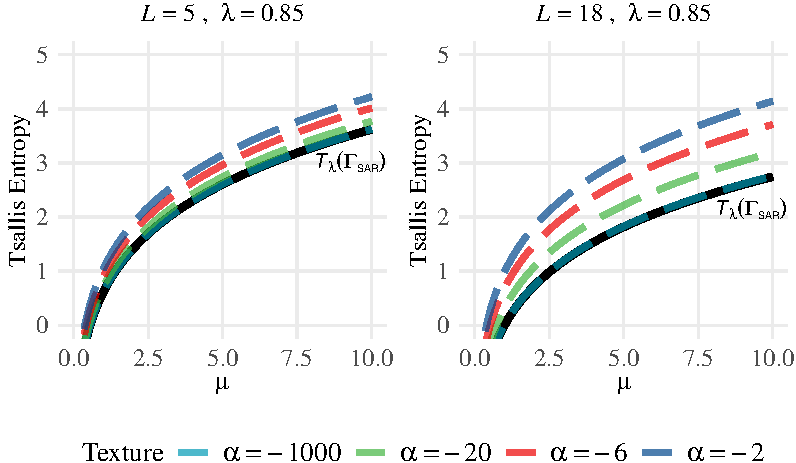
\includegraphics[keepaspectratio]{Figures/fig-tsallis-convergence_L18-1.pdf}}

}

\caption{\label{fig-tsallis-convergence_L18}Tsallis entropy
\(T_{\lambda}(\mathcal{G}^0_I)\) converges to
\(T_{\lambda}(\Gamma_{\mathrm{SAR}})\) as \(\alpha\) decreases.}

\end{figure}%

For the highly heterogeneous case (\(\alpha=-2\)), entropy values are
very similar for \(L=5\) and \(L=18\), since texture dominates over
speckle. In contrast, in the homogeneous limit (\(\alpha \to -\infty\)),
texture effects vanish and entropy is mainly determined by speckle. With
a low number of looks, speckle is strong and increases the uncertainty,
which raises the entropy values. However, the curves for different
\(\alpha\) values appear more concentrated, since the contribution of
texture to entropy is masked by the dominant speckle. As the number of
looks increases, speckle is progressively reduced and entropy decreases.
This reduction of speckle makes the excess entropy \(\Delta_\alpha\)
more evident, resulting in more separated curves across \(\alpha\).

\subsection{Non-parametric Estimation of Tsallis
Entropy}\label{non-parametric-estimation-of-tsallis-entropy}

\label{subsec:tsallis-np}

Following the spacing-based approach of
Vasicek~\citeproc{ref-vasicek1976test}{{[}20{]}} and Ebrahimi et
al.~\citeproc{ref-Ebrahimi1994}{{[}21{]}} for Shannon entropy, and the
methodology for Rényi entropy proposed by Al-Labadi et
al.~\citeproc{ref-AlLabadi2024}{{[}22{]}}, we derive a nonparametric
estimator for Tsallis entropy.

Let \(Q(p)=F^{-1}(p)\) denote the quantile function for \(p\in(0,1)\).
From \eqref{eq:tsallis}, the inner integral can be expressed as an
expectation under \(Z\sim f\): \[
\int_{\mathcal B} f(z)^\lambda\,\mathrm{d}z
=\int_{\mathcal B} f(z)^{\lambda-1} f(z)\,\mathrm{d}z
=\mathbb{E}\!\left[f(Z)^{\lambda-1}\right].
\] Using the change of variables \(p=F(z)\) (hence
\(\mathrm{d}p=f(z)\,\mathrm{d}z\)) and the identity \(f(Q(p))=1/Q'(p)\),
we obtain \[
  \mathbb{E}\!\left[f(Z)^{\lambda-1}\right]
  = \int_{0}^{1} \bigl(Q'(p)\bigr)^{1-\lambda}\,\mathrm{d}p,
\] which yields the representation \begin{equation}
  T_\lambda(Z)
  =\frac{1}{\lambda-1}
     \left\{
       1-\int_{0}^{1}\bigl(Q'(p)\bigr)^{1-\lambda}\,\mathrm{d}p
     \right\}.
  \label{eq:Tsallis-quantile}
\end{equation} Let \(\bm{Z}=(Z_1,\dots,Z_n)\) be an i.i.d.~sample from
\(F\), with order statistics \(Z_{(1)}\le\cdots\le Z_{(n)}\). For a
window size \(m\in\{1,\dots,\lfloor (n-1)/2\rfloor\}\), define the
\(m\)-spacing \[
D_{i,m}:=Z_{(i+m)}-Z_{(i-m)},\qquad i=1,\dots,n,
\] with boundary conventions \(Z_{(i-m)}:=Z_{(1)}\) if \(i\le m\) and
\(Z_{(i+m)}:=Z_{(n)}\) if \(i\ge n-m\). The \(m\)-spacing density
estimator at \(Z_{(i)}\) is \begin{equation}
\widehat f_n\bigl(Z_{(i)}\bigr)
=\frac{c_i\, (m/n)}{Z_{(i+m)}-Z_{(i-m)}}\,,\qquad i=1,\dots,n,
\label{eq:density-spacing}
\end{equation} where \[
c_i=
\begin{cases}
\dfrac{m+i-1}{m}, & 1\le i\le m,\\[6pt]
2, & m+1\le i\le n-m,\\[6pt]
\dfrac{n+m-i}{m}, & n-m+1\le i\le n.
\end{cases}
\] By construction, \(\widehat f_n(Z_{(i)})\approx f(Z_{(i)})\). Since
\(f(Q(p))\,Q'(p)=1\), taking the reciprocal yields an estimator of the
quantile derivative: \begin{equation}
\widehat{Q'}(p_i)
\;=\; \frac{1}{\widehat f_n(Z_{(i)})}
\;=\; \frac{D_{i,m}}{c_i\, (m/n)}\,,
\qquad p_i \in (0,1).
\label{eq:Qprime-hat}
\end{equation} Approximating the integral in \eqref{eq:Tsallis-quantile}
by a Riemann sum over the grid \(p_i=i/n\) and inserting
\(\widehat{Q'}(p_i)\) from \eqref{eq:Qprime-hat} yields the
nonparametric Tsallis entropy estimator: \begin{align}
  \widehat T_{\lambda}(\bm{Z})
  &=\frac{1}{\lambda-1}\left\{
1-\frac{1}{n}\sum_{i=1}^{n}\bigl[\widehat{Q'}(p_i)\bigr]^{\,1-\lambda}
\right\}, \nonumber\\[4pt]
  &= \frac{1}{\lambda-1}
  \left\{
    1-\frac{1}{n}
       \sum_{i=1}^{n}
       \left(
         \frac{Z_{(i+m)}-Z_{(i-m)}}{c_i\, (m/n)}
       \right)^{1-\lambda}
  \right\}.
  \label{eq:Tsallis-spacing-estimator}
\end{align} As \(\lambda\to 1\), \(T_\lambda\) converges to Shannon
entropy and \(\widehat T_{\lambda}\) recovers the Vasicek
estimator~\citeproc{ref-vasicek1976test}{{[}20{]}}. This estimator is
asymptotically consistent, i.e., it converges in probability to the true
value when \(m,n\rightarrow\infty\) and \(m/n\rightarrow0\). We use the
heuristic spacing \(m=\left[\sqrt{n}+0.5\right]\).

\section{PROPOSED METHODOLOGY}\label{sec:met}

\subsection{\texorpdfstring{Finding an optimal value of
\(\lambda\)}{Finding an optimal value of \textbackslash lambda}}\label{finding-an-optimal-value-of-lambda}

We aim to determine the optimal order \(\lambda\) for the Tsallis
entropy estimator using simulated samples of size \(n = 49\) from
\(Z\sim \Gamma_{\text{SAR}}(5,1)\). We computed the bias and the mean
squared error (MSE) for varying \(\lambda\) via a Monte Carlo
experiment.

As shown in Fig.~\ref{fig-optimal_order-tsallis}, for \(L>1\) we found
that \(\lambda=0.85\) yields the lowest MSE while maintaining a low
bias, thus providing a favorable trade-off between bias and variance.

\begin{figure}[H]

\centering{

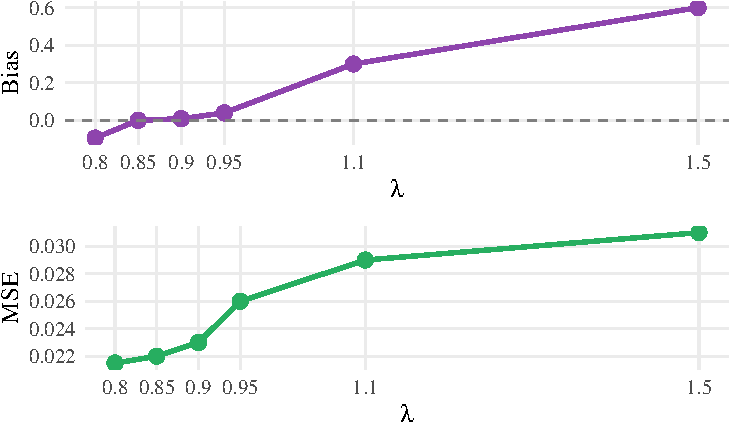
\includegraphics[width=0.95\linewidth,height=\textheight,keepaspectratio]{Figures/fig-optimal_order-tsallis-1.pdf}

}

\caption{\label{fig-optimal_order-tsallis}Bias and MSE as a function of
\(\lambda\), for the Tsallis entropy estimator, with \(n = 49\),
\(L = 5\).}

\end{figure}%

\subsection{Bootstrap Correction for Entropy
Estimator}\label{bootstrap-correction-for-entropy-estimator}

Following
Refs.~\citeproc{ref-Frery2024}{{[}23{]}}--\citeproc{ref-Alpala2025}{{[}25{]}},
we refine the non-parametric entropy estimator \(\widehat{T}_{\lambda}\)
in~\eqref{eq:Tsallis-spacing-estimator} with bootstrap, obtaining
\(\widetilde{T}_{\lambda}\): \begin{equation*}
\widetilde{T}_{\lambda} = 2\widehat{T}_{\lambda}(\bm{Z}) - \frac{1}{B} \sum_{b=1}^{B} \widehat{T}_{\lambda}(\bm{Z}^{(b)}),
\end{equation*} where \(B\) is the number of bootstrap replications, and
\(\bm{Z}^{(b)}\) denotes the \(b\)-th resampled dataset obtained by
drawing \(n\) observations with replacement from \(\bm{Z}\).

A Monte Carlo study with \(1000\) replications for each sample size
\(n \in \{9, 25, 49, 81, 121\}\) from the \(\Gamma_{\text{SAR}}\) (5,1)
confirms that for \(\lambda=0.85\), the bootstrap-corrected estimator
\(\widetilde{T}_{\lambda}\) (\(B=200\)) reduces both bias and MSE
compared to the original \(\widehat{T}_{\lambda}\), with significant
improvements for small sample sizes, as shown in
Fig.~\ref{fig-bias_mse_Tsallis}.

\begin{figure}[H]

\centering{

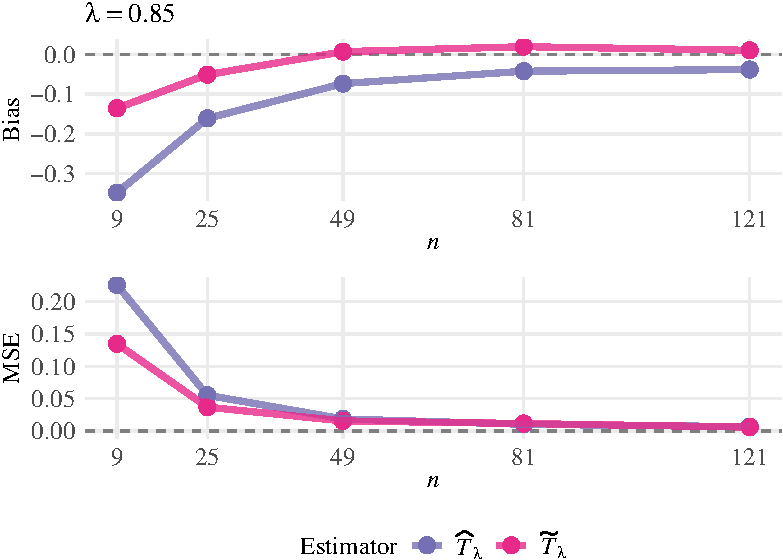
\includegraphics[width=0.9\linewidth,height=\textheight,keepaspectratio]{Figures/fig-bias_mse_Tsallis-1.pdf}

}

\caption{\label{fig-bias_mse_Tsallis}Bias and MSE of the Tsallis entropy
estimators for \(\Gamma_{\text{SAR}}\), with \(L=5\)}

\end{figure}%

From this point forward, all subsequent simulations and comparisons will
be based on the improved bootstrap estimator:
\(\widetilde{T}_{\lambda}\).

\subsection{Hypothesis Testing}\label{hypothesis-testing}

We test whether the observed data come from a homogeneous
(\(\Gamma_{\text{SAR}}\)) or a heterogeneous (\(\mathcal{G}^0_I\))
region, as follows: \begin{equation}\label{eq:hypothesis_test}
\begin{cases}
\mathcal{H}_0: \mathbb{E}[\widetilde{T}_{\lambda}] = T_{\lambda}(\Gamma_{\text{SAR}}) & \text{(Homogeneous region)}, \\[6pt]
\mathcal{H}_1: \mathbb{E}[\widetilde{T}_{\lambda}] = T_{\lambda}(\mathcal{G}^0_I) & \text{(Heterogeneous region)}.
\end{cases}
\end{equation}

Under \(\mathcal{H}_0\), the expected value of the entropy estimator
should match the theoretical \(T_{\lambda}(\Gamma_{\text{SAR}})\).
Significant deviations indicate heterogeneity.

\subsection{The Proposed Test}\label{the-proposed-test}

We propose a test statistic that identifies the discrepancy between
estimated and theoretical entropy under homogeneity. Since \(L\geq1\) is
known, we define the test statistic as follows: \begin{multline}
\label{eq-test-tsallis}
S_{\widetilde{T}_{\lambda}}(\bm{Z}; L) = \widetilde{T}_{\lambda} - \biggl\{ \frac{1}{\lambda - 1} \Bigl[ 1 -
\exp\Bigl(
(1 - \lambda)\ln \widehat{\mu}\\
+ (\lambda - 1)\ln L
+ \ln\Gamma\bigl(\lambda(L - 1) + 1\bigr) \\
- \lambda\ln\Gamma(L)
- \bigl(\lambda(L - 1) + 1\bigr)\ln \lambda
\Bigr) \Bigr] \biggr\},
\end{multline} where \(\widehat{\mu} = \frac{1}{n} \sum_{i=1}^n Z_i\) is
the sample mean.

This statistic can be interpreted as: \[
S_{\widetilde T_\lambda} 
= 
\underbrace{\widetilde T_\lambda}_{\text{estimated}} 
\;-\;
\underbrace{T_\lambda\bigl(\Gamma_{\mathrm{SAR}}\bigr)}_{\text{theoretical under } H_0}\hspace{-0.5em},
\] the difference between the estimated entropy and the expected value
under homogeneity. Values close to zero indicate that the region behaves
like fully developed speckle, while large positive values signal excess
entropy and, thus, heterogeneity. This formulation avoids the need to
estimate \(\mathcal{G}^0_I\) parameters such as \(\alpha\), offering a
simple, interpretable, and statistically grounded test. Moreover, the
method remains effective for small samples, aided by the bootstrap bias
correction.

Fig. \ref{fig-densities-tsallis4} shows the empirical distribution of
\(S_{\widetilde{T}_{\lambda}}\) under \(\mathcal{H}_0\), obtained from
\(10^4\) Monte Carlo simulations with varying sample sizes
(\(n \in \{49,81,121\}\)), \(\lambda = 0.85\), and \(L \in \{5,18\}\).
The empirical densities are tightly concentrated around zero, confirming
that under \(\mathcal{H}_0\) the test statistic has mean approximately
\(0\); at the same time, their moderately heavy tails reveal sensitivity
to departures from homogeneity, which is desirable for detecting subtle
texture.

\begin{figure}[H]

\centering{

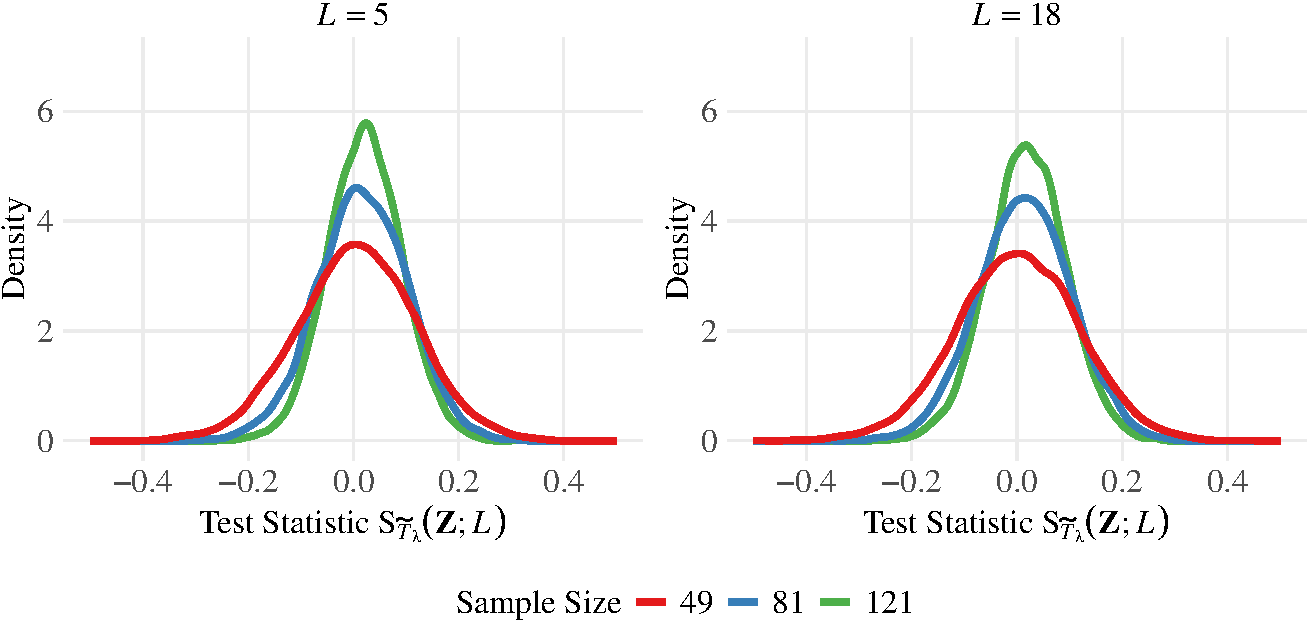
\includegraphics[width=0.99\linewidth,height=\textheight,keepaspectratio]{Figures/fig-densities-tsallis4-1.pdf}

}

\caption{\label{fig-densities-tsallis4}Empirical densities of
\(S_{\widetilde{T}_{\lambda}}(\bm{Z}; L)\) under \(\mathcal{H}_0\), with
\(\lambda=0.85\).}

\end{figure}%

Under the asymptotic properties of the entropy estimators
\citeproc{ref-vasicek1976test}{{[}20{]}},
\citeproc{ref-VanEs1992}{{[}26{]}}, for sufficiently large samples,
\(S_{\widetilde{T}}(\bm{Z};L)\) follows an asymptotic normal
distribution: \[
  S_{\widetilde{T}}(\mathbf Z;L)\;
  \overset{\mathcal{D}}{\underset{n \to \infty}{\longrightarrow}}\;
  \mathcal N\!\bigl(\mu_S,\sigma_S^{2}\bigr),
\] where \(\xrightarrow{\mathcal{D}}\) denotes convergence in
distribution.

Here, \(\mu_S = \mathbb{E}[S_{\widetilde{T}}(\bm{Z};L)]\) and
\(\sigma^2_S = \mathrm{Var}[S_{\widetilde{T}}(\bm{Z};L)]\) are the
theoretical mean and variance of the test statistic under
\(\mathcal{H}_0\). This asymptotic normality can be explained by noting
that the entropy estimator (and hence \(S_{\widetilde{T}}\)) can be
expressed as a sum or average of numerous observations; therefore, by
the Central Limit Theorem and the delta method, its sampling
distribution approaches a Gaussian form for large \(n\).

In practice, we estimate \(\widehat{\mu}_S\) and \(\widehat{\sigma}_S\)
via Monte Carlo under \(\mathcal{H}_0\). \begin{equation*}
\varepsilon = \frac{{S_{\widetilde{T}}(\bm{Z}; L) - \widehat{\mu}_S}}{{\widehat{\sigma}_S}},
\end{equation*} which is asymptotically standard normal distributed for
large \(n\). Consequently, two-sided \(p\)-values are obtained as
\(2\Phi(-|\varepsilon|)\), where \(\Phi(\cdot)\) is the cumulative
distribution function of the standard normal distribution.

The practical procedure is as follows: first, compute the test statistic
\(S_{\widetilde{T}}(\bm{Z}; L)\) for the observed data; then standardize
it using the estimated mean and standard deviation
\((\widehat{\mu}_S, \widehat{\sigma}_S)\); next, compute the \(p\)-value
as \(2\Phi(-|\varepsilon|)\); and finally, make a decision by comparing
the \(p\)-value with the threshold \(0.05\), as illustrated in
Fig.~\ref{fig:entropy-diagram-test}.

\begin{figure}[H]
    \centering
\begin{tikzpicture}[
  node distance=1.5cm and 1.5cm,
  box/.style={
    rectangle, draw=black, fill=teal!20,
    minimum width=3.5cm, minimum height=1.2cm,
    align=center, font=\small, text=black, font=\bfseries
  },
  arrow/.style={
    -{Stealth[length=2mm, width=1.2mm]},
    semithick
  }
]
  % fila superior
  \node[box] (raw) {1. Calculate\\test statistic\\ $S(\bm{Z})$};
  \node[box,right=of raw] (std) {2. Standardize\\test statistic\\ $\varepsilon=(S-\hat\mu_S)/\hat\sigma_S$};
  
  % fila inferior
  \node[box,below=of raw] (pval) {4. Make decision\\Reject if\\ $p<0.05$};
  \node[box,right=of pval] (dec) {3. Compute \\ $p$-value \\ $2\Phi(-|\varepsilon|)$};

  % flechas
  \draw[arrow] (raw.east) -- (std.west);
  \draw[arrow] (std.south) -- (dec.north);   % de 2 hacia abajo al 4
  \draw[arrow] (dec.west) -- (pval.east);    % de 4 a 3
 % \draw[arrow] (pval.north) -- (raw.south);  % de 3 hacia arriba al 1 (opcional, si quieres ciclo)
\end{tikzpicture}
    \caption{Workflow of the entropy‐based hypothesis test.}
    \label{fig:entropy-diagram-test}
\end{figure}

\subsection{Size and Power Analysis of the Proposed
Test}\label{size-and-power-analysis-of-the-proposed-test}

The statistical validity and effectiveness of the proposed Tsallis
entropy--based test was examined through two fundamental properties:
\emph{size} and \emph{power}. These provide insight into the probability
of incorrect decisions in hypothesis testing.

The size of a statistical test, also known as the Type~I~error rate,
refers to the probability of incorrectly rejecting the null hypothesis
\(\mathcal{H}_0\) when it is in fact true. In hypothesis testing,
practitioners typically specify a nominal significance level, commonly
set at \SI{1}{\percent}, \SI{5}{\percent}, and \SI{10}{\percent}, which
represent acceptable probabilities of committing a Type~I error. A
well-calibrated test should reproduce these levels empirically across
sample sizes and conditions.

To assess this, we performed \(1000\) Monte Carlo replications under
\(\mathcal{H}_0\) with data from a \(\Gamma_{\text{SAR}}\) distribution
(\(\mu=1\)), computing the test statistic via a bootstrap entropy
estimator (\(B=100\), \(\lambda=0.85\)). The empirical size was then
estimated as the proportion of replications in which the null hypothesis
was incorrectly rejected. The observed Type~I error rates remained close
to the nominal levels, confirming the validity and proper calibration of
the proposed procedures.

The power of a test is its probability of correctly rejecting
\(\mathcal{H}_0\) when it is false. Equivalently, it equals \(1-\beta\),
where \(\beta\) is the Type~II error rate. High power thus indicates
strong sensitivity to departures from \(\mathcal{H}_0\). To assess
power, we simulated data under the alternative hypothesis
\(\mathcal{H}_1\), assuming a \(\mathcal{G}^0_I\) distribution with
\(\mu=1\) and \(\alpha=-2\). Again, \(1000\) Monte Carlo replications
were performed for each configuration of sample size and \(L\), and the
test statistic was computed using the bootstrap estimator (\(B=100\),
\(\lambda=0.85\)).

As expected, power increased with both the sample size and the number of
looks, confirming the effectiveness of the Tsallis entropy--based test
in detecting departures from the null hypothesis.

The complete results for both size and power are reported in Table
\ref{tab:size-power-tsallis}.

\renewcommand{\arraystretch}{1}
\begin{table}[H]
\centering\centering
\caption{\label{tab:size-power-tsallis}Size and Power of the $S_{\widetilde{T}_{\lambda}}(\bm{Z})$ test statistic (Tsallis).}
\resizebox{\ifdim\width>\linewidth\linewidth\else\width\fi}{!}{
\fontsize{10}{12}\selectfont
\begin{tabu} to \linewidth {>{\centering}X>{\centering}X>{\centering}X>{\centering}X>{\centering}X>{\centering}X>{\centering}X>{\centering}X}
\toprule
\multicolumn{2}{c}{ } & \multicolumn{3}{c}{Size} & \multicolumn{3}{c}{Power} \\
\cmidrule(l{3pt}r{3pt}){3-5} \cmidrule(l{3pt}r{3pt}){6-8}
\multicolumn{1}{c}{$\bm{L}$} & \multicolumn{1}{c}{$\bm{n}$} & \multicolumn{1}{c}{$\hphantom{00}\SI{1}{\percent}$} & \multicolumn{1}{c}{$\hphantom{00}\SI{5}{\percent}$} & \multicolumn{1}{c}{$\hphantom{00}\SI{10}{\percent}$} & \multicolumn{1}{c}{$\hphantom{00}\SI{1}{\percent}$} & \multicolumn{1}{c}{$\hphantom{00}\SI{5}{\percent}$} & \multicolumn{1}{c}{$\hphantom{00}\SI{10}{\percent}$}\\
\midrule
 & 25 & $\phantom{-}0.014$ & $\phantom{-}0.051$ & $\phantom{-}0.103$ & $\phantom{-}0.958$ & $\phantom{-}0.991$ & $\phantom{-}0.990$\\

 & 49 & $\phantom{-}0.011$ & $\phantom{-}0.048$ & $\phantom{-}0.107$ & $\phantom{-}0.990$ & $\phantom{-}1.000$ & $\phantom{-}0.999$\\

 & 81 & $\phantom{-}0.012$ & $\phantom{-}0.057$ & $\phantom{-}0.101$ & $\phantom{-}0.997$ & $\phantom{-}0.998$ & $\phantom{-}0.999$\\

\multirow{-4}{*}[1.5\dimexpr\aboverulesep+\belowrulesep+\cmidrulewidth]{\centering\arraybackslash 5} & 121 & $\phantom{-}0.014$ & $\phantom{-}0.060$ & $\phantom{-}0.116$ & $\phantom{-}0.999$ & $\phantom{-}0.999$ & $\phantom{-}0.997$\\
\cmidrule{1-8}
 & 25 & $\phantom{-}0.010$ & $\phantom{-}0.049$ & $\phantom{-}0.108$ & $\phantom{-}0.992$ & $\phantom{-}1.000$ & $\phantom{-}1.000$\\

 & 49 & $\phantom{-}0.008$ & $\phantom{-}0.055$ & $\phantom{-}0.108$ & $\phantom{-}1.000$ & $\phantom{-}0.999$ & $\phantom{-}1.000$\\

 & 81 & $\phantom{-}0.012$ & $\phantom{-}0.052$ & $\phantom{-}0.097$ & $\phantom{-}0.998$ & $\phantom{-}1.000$ & $\phantom{-}0.999$\\

\multirow{-4}{*}[1.5\dimexpr\aboverulesep+\belowrulesep+\cmidrulewidth]{\centering\arraybackslash 8} & 121 & $\phantom{-}0.016$ & $\phantom{-}0.072$ & $\phantom{-}0.116$ & $\phantom{-}0.998$ & $\phantom{-}1.000$ & $\phantom{-}0.999$\\
\cmidrule{1-8}
 & 25 & $\phantom{-}0.015$ & $\phantom{-}0.052$ & $\phantom{-}0.111$ & $\phantom{-}1.000$ & $\phantom{-}1.000$ & $\phantom{-}1.000$\\

 & 49 & $\phantom{-}0.013$ & $\phantom{-}0.046$ & $\phantom{-}0.099$ & $\phantom{-}1.000$ & $\phantom{-}1.000$ & $\phantom{-}1.000$\\

 & 81 & $\phantom{-}0.013$ & $\phantom{-}0.047$ & $\phantom{-}0.105$ & $\phantom{-}1.000$ & $\phantom{-}1.000$ & $\phantom{-}1.000$\\

\multirow{-4}{*}[1.5\dimexpr\aboverulesep+\belowrulesep+\cmidrulewidth]{\centering\arraybackslash 18} & 121 & $\phantom{-}0.012$ & $\phantom{-}0.065$ & $\phantom{-}0.109$ & $\phantom{-}1.000$ & $\phantom{-}1.000$ & $\phantom{-}1.000$\\
\bottomrule
\end{tabu}}
\end{table}

\subsection{Adaptive Windows with Tsallis
Entropy}\label{adaptive-windows-with-tsallis-entropy}

Our approach builds on the adaptive windowing algorithm for SAR images
proposed by Park et al. \citeproc{ref-Park1999}{{[}17{]}}, which adjusts
the analysis window size according to the local homogeneity of the
scene. For each pixel \((i,j)\), the coefficient of variation is
computed over the border of the current window, \begin{equation}
C_{ij} = \frac{\sigma_{ij}}{\mu_{ij}},
\end{equation} where \(\mu_{ij}\) and \(\sigma_{ij}\) are calculated
using only the border pixels \(b_{ij}\) of the window \(w_{ij}\). In
homogeneous areas, \(C_{ij} \approx \sigma_n\), with \begin{equation}
\sigma_n = \frac{0.523}{\sqrt{L}}.
\end{equation} The homogeneity criterion is defined by comparing
\(C_{ij}\) with an adaptive threshold \(U_{ij}\), given by
\begin{equation}
U_{ij} = \eta\left( 1 + \sqrt{\frac{1 + 2\sigma_n^2}{8(W_{ij} - 1)}} \right)\sigma_n,
\end{equation} where \(W_{ij} = 2N_{ij} + 1\) is the current window side
length (with radius \(N_{ij}\)), and \(\eta\) is a tuning parameter
controlling the degree of smoothing. Values close to \(\eta=1.0\)
provide limited speckle suppression, while larger values increase
smoothing and yield stronger noise reduction.

The window radius \(N_{ij}\) is updated dynamically and locally as
follows: \[
N_{i,j+1} =
\begin{cases}
\min(N_{ij} + 1, N_{\max}), & \text{if } C_{ij} \leq U_{ij}, \\
\max(N_{ij} - 1, N_{\min}), & \text{if } C_{ij} > U_{ij},
\end{cases}
\] here, \(N_{\max}\) and \(N_{\min}\) denote the maximum and minimum
window size, respectively.

The procedure can be summarized as:

\begin{itemize}
\tightlist
\item
  \textbf{Homogeneous regions} (\(C_{ij} \leq U_{ij}\)): the window
  grows, up to \(N_{\max}\), which enhances speckle reduction and
  stabilizes the estimates.\\
\item
  \textbf{Heterogeneous regions} (\(C_{ij} > U_{ij}\)): the window
  shrinks, down to \(N_{\min}\), which preserves edges and prevents the
  mixing of different classes.
\end{itemize}

Once the window radius \(N_{ij}\) has been determined for pixel
\((i,j)\), the corresponding full window is extracted and the proposed
test in \eqref{eq-test-tsallis} is applied to obtain the local
statistic. This produces two outputs:

\begin{itemize}
\tightlist
\item
  a map of test statistics over the image, and\\
\item
  a window-size map \(W_{ij}\), which records the locally selected
  window side (larger in homogeneous regions, smaller in heterogeneous
  ones).
\end{itemize}

For inference, each value of the test statistic is standardized using
the empirical mean and standard deviation of the image, and two-sided
\(p\)-values are then computed.

This adaptive strategy has several advantages. It is locally responsive
to image texture, using small windows in heterogeneous areas and larger
ones in homogeneous zones. This ensures edge preservation and
statistical stability, while the parameter \(\eta\) controls the balance
between smoothness and detail preservation. Moreover, the framework is
extensible and can be applied with any entropy estimator.

\section{RESULTS}\label{sec:app}

\subsection{Analysis with Simulated Data}\label{sec-sim2}

Figure~\ref{fig:sim_Phantom_1} presents the structural design of the
synthetic phantom with dimensions of \(500\times500\) pixels, proposed
by Gomez et al.~\citeproc{ref-Gomez2017}{{[}27{]}} as a tool to assess
the performance of speckle-reduction filters. This layout serves as a
base template to generate the simulated images shown in
Figures~\ref{fig:sim_Phantom_2}.

Each region is filled with data simulated from the \(\mathcal{G}^0_I\)
distribution~\eqref{E:gi02}, using different combinations of the
roughness parameter \(\alpha\) and the mean \(\mu\), as indicated by the
labels in each quadrant of the image. Light regions correspond to
textured observations (heterogeneous), while darker regions represent
textureless areas (homogeneous).

The \(\alpha\) parameter of the \(G_I^0\) distribution is essential for
interpreting texture characteristics. Values near zero greater than
\(-3\) suggest extremely textured targets, such as urban
zones~\citeproc{ref-Frery2019a}{{[}28{]}}. As the value decreases, it
indicates regions with moderate texture (in the \(\left[-6,-3\right]\)
region), related to forest zones, while values below \(-6\) correspond
to textureless regions, such as pasture, agricultural fields, and water
bodies~\citeproc{ref-Neto2023}{{[}29{]}}.

The proposed Tsallis-based test statistic,
\(S_{\widetilde{T}_\lambda}\), was applied to the simulated image using
the adaptive windowing strategy with side lengths ranging from
\(5\times 5\) (minimum) to \(11\times 11\) (maximum), with the smoothing
parameter set to \(\eta = 5\). Figure~\ref{fig:pvalueL9} displays the
resulting \(p\)-value map for \(L=9\).

\begin{figure*}[hbt]
    \centering
     \begin{subfigure}{0.25\textwidth}
        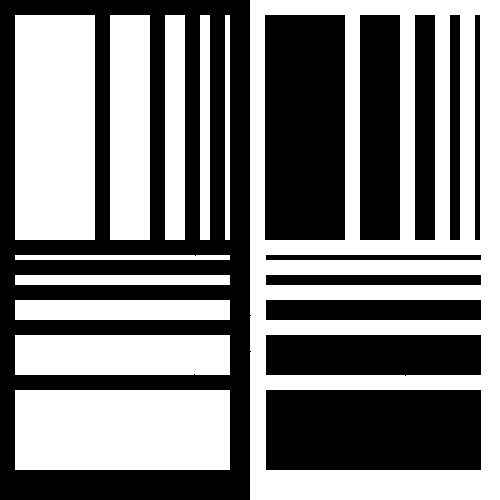
\includegraphics[width=\linewidth]{./Figures/Phantom1.png}
        \caption{Phantom}
        \label{fig:sim_Phantom_1}
    \end{subfigure}
   \hspace{0.00001\textwidth}
    \begin{subfigure}{0.35\textwidth}
        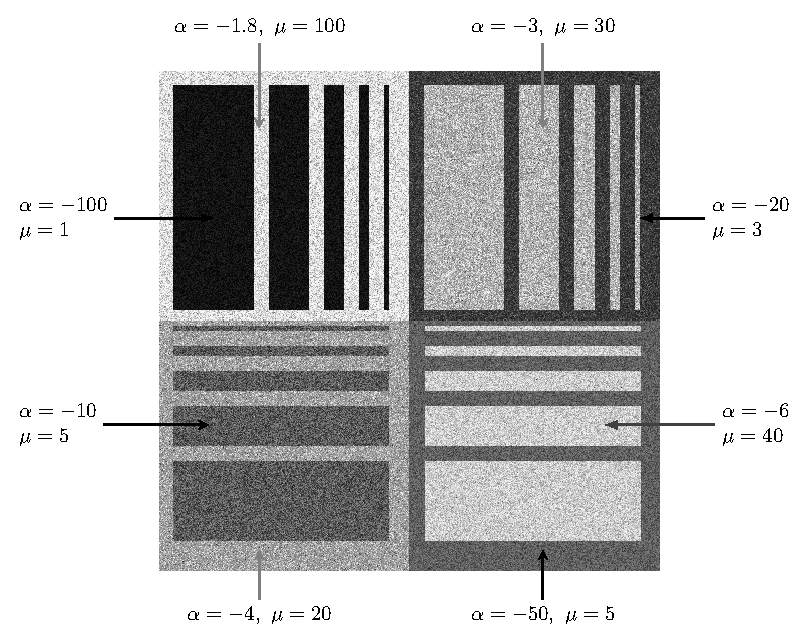
\includegraphics[width=\linewidth]{./Figures/Phantom4_L9.pdf}
        \caption{Simulated image}
        \label{fig:sim_Phantom_2}
    \end{subfigure}
   \hspace{0.00001\textwidth}
    \begin{subfigure}{0.32\textwidth}
        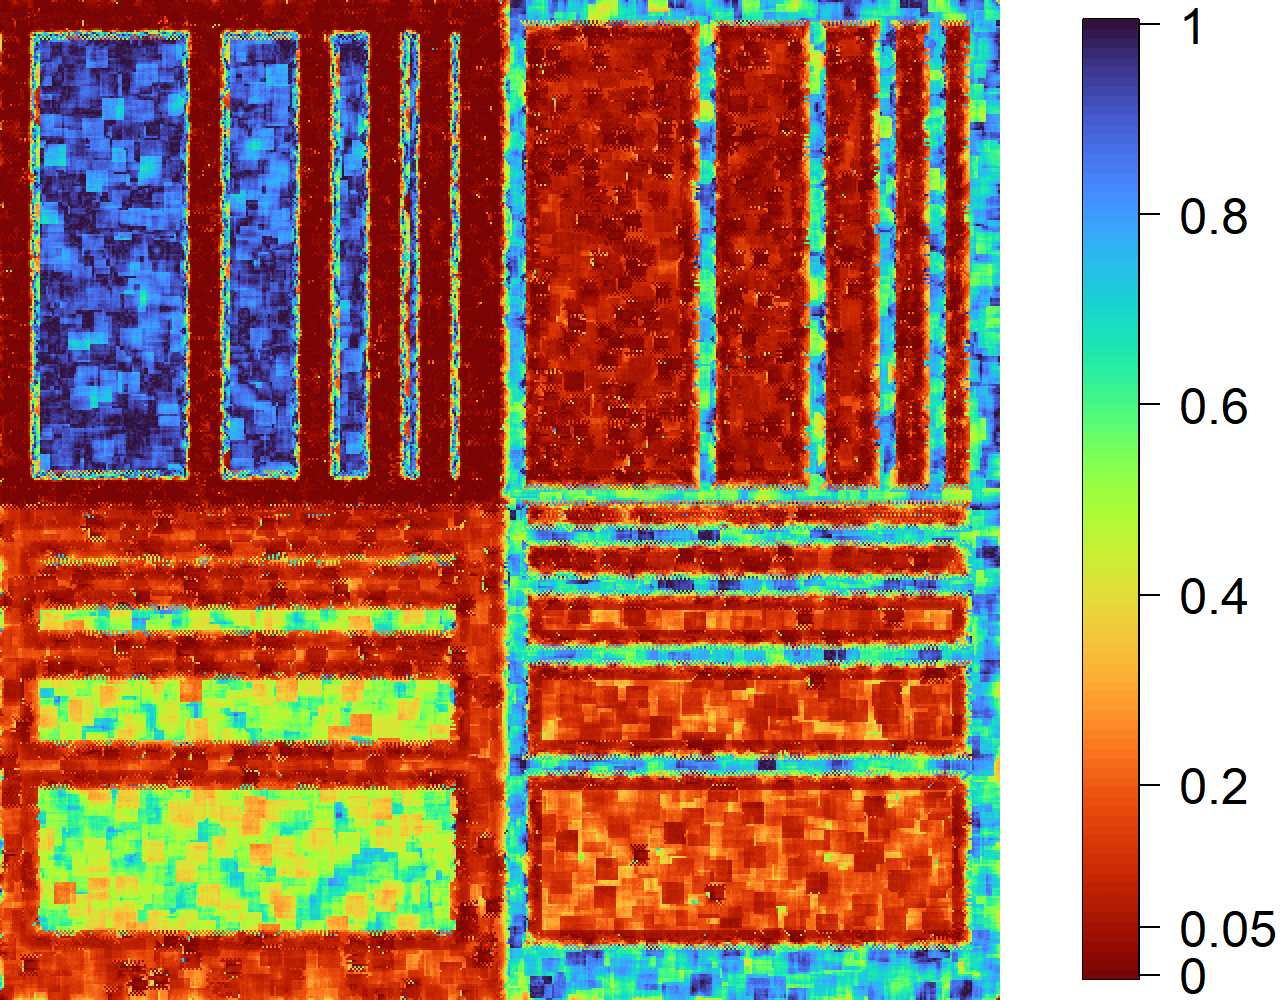
\includegraphics[width=\linewidth]{./Figures/p-values_tsallis_L9_B200_eta_5_5x11_085_inv.png}
        \caption{$p$-value map  }
        \label{fig:pvalueL9}
    \end{subfigure}
    \caption{Results on simulated data using the test statistic $S_{\widetilde{T}_{\lambda}}$ with adaptive windows ranging from $5\times5$ to $11\times11$. The image has size $500\times500$ pixels, with $L=9$.}

    \label{fig:simL9}
\end{figure*}

The color gradient provides an interpretable scale: dark red regions
(\(p \approx 0\)) indicate strong evidence of heterogeneity,
consistently appearing in highly textured zones such as those with
\(\alpha > -3\), while dark blue regions (\(p \approx 1\)) correspond to
homogeneous areas, typically observed for very low \(\alpha\) values
(e.g., \(\alpha < -6\)). Intermediate colors, such as yellow and green
(\(p \approx 0.2\)--\(0.6\)), represent transitional responses that
capture moderately textured areas (e.g., \(-6 \leq \alpha \leq -3\)),
whereas light blue tones (\(p \approx 0.7\)--\(0.9\)) occur in regions
that are close to homogeneous but still contain subtle texture
variations. This gradation of colors highlights the sensitivity of the
proposed test: instead of producing only binary outcomes, it provides a
continuous measure of heterogeneity across the image, allowing areas
with intermediate texture levels to be represented by intermediate
\(p\)-values that reflect the gradual transition between homogeneous and
heterogeneous scattering conditions.

\subsection{Applications to SAR Data}\label{applications-to-sar-data}

The selected scenes, acquired in HH polarization, correspond to the
outskirts of Munich and Dublin Port (Ireland), as shown in
Figs.~\ref{fig:munich-sar}-\ref{fig:dublin-sar}. Corresponding optical
images (Figs.~\ref{fig:munich-o}--\ref{fig:dublin-o}) illustrate land
cover context.

Table~\ref{tab:table_param} details the SAR acquisition parameters.
\renewcommand{\arraystretch}{2.5}

\begin{table}[H]
\centering\centering
\caption{\label{tab:table_param}Parameters of selected SAR images}
\centering
\resizebox{\ifdim\width>\linewidth\linewidth\else\width\fi}{!}{
\fontsize{22}{24}\selectfont
\begin{tabu} to \linewidth {>{\centering\arraybackslash}p{3.0cm}>{\centering\arraybackslash}p{4.5cm}>{\centering\arraybackslash}p{1.5cm}>{\centering\arraybackslash}p{4cm}>{\centering\arraybackslash}p{1.5cm}>{\centering\arraybackslash}p{4.0cm}>{\centering\arraybackslash}p{4.5cm}}
\toprule
\multicolumn{1}{c}{\textbf{Scene}} & \multicolumn{1}{c}{\textbf{Mission}} & \multicolumn{1}{c}{\textbf{Band}} & \multicolumn{1}{c}{\textbf{Size (pixels)}} & \multicolumn{1}{c}{$\bm{L}$} & \multicolumn{1}{c}{\textbf{Resolution [m]}} & \multicolumn{1}{c}{\textbf{Acquisition Date}}\\
\midrule
Munich & UAVSAR & L & $1024\times1024$ & $12$ & $4.9\times7.2$ & 16-04-2015\\
Dublin & TanDEM-X & X & $1100\times1100$ & $16$ & $1.35\times1.35$ & 03-09-2017\\
\bottomrule
\end{tabu}}
\end{table}

We applied the proposed test statistic \(S_{\widetilde{T}_{\lambda}}\)
to real SAR data using adaptive local sliding windows ranging from
\(5 \times 5\) to \(11 \times 11\), with the smoothing parameter set to
\(\eta = 5\). The results are illustrated in
Figures~\ref{fig:munichp}--\ref{fig:dublinp}, which display the original
SAR image, the corresponding optical reference, and the resulting
\(p\)-value maps.

\begin{figure*}[hbt]
    \centering
    \begin{subfigure}{0.25\textwidth}
        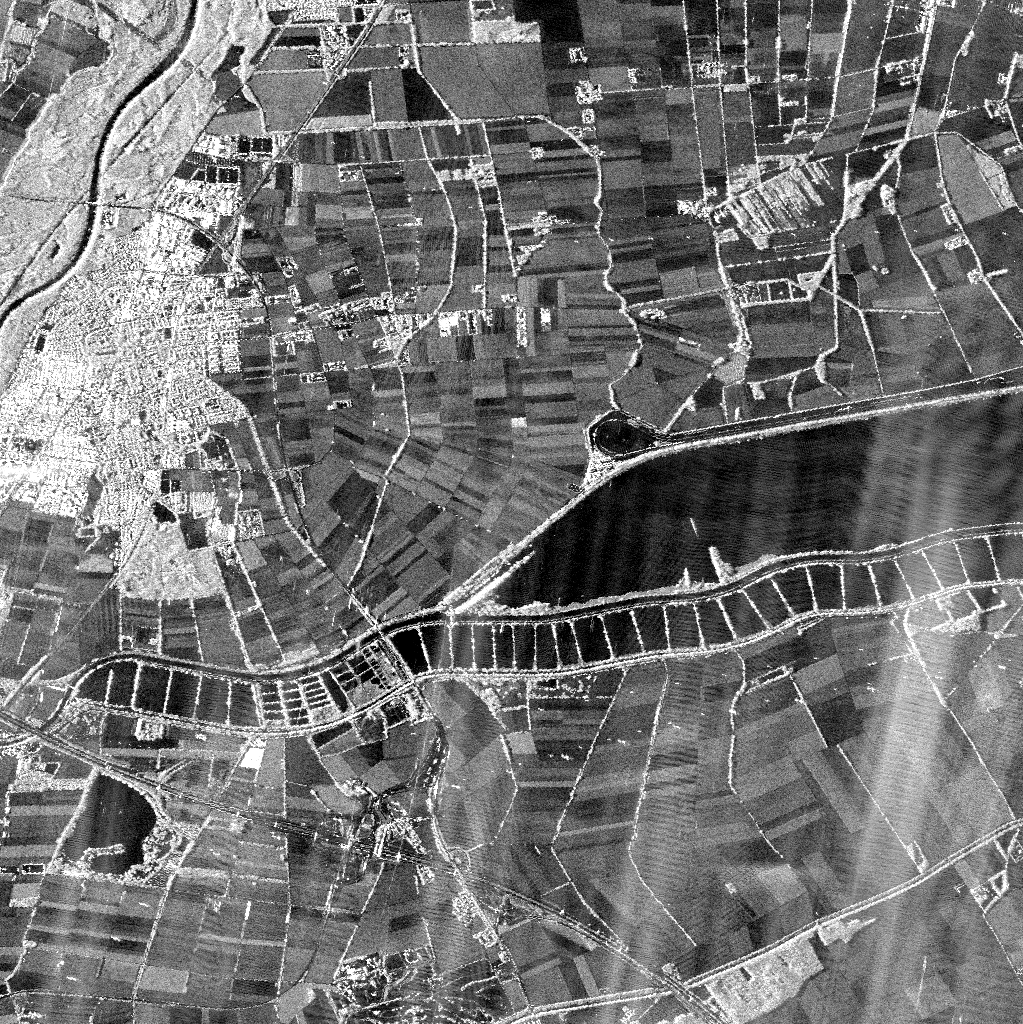
\includegraphics[width=\linewidth]{./Figures/munich_1024.png}
        \caption{Simulated image}
        \label{fig:munich-sar}
    \end{subfigure}
        \hspace{0.001\textwidth}
    \begin{subfigure}{0.235\textwidth}
        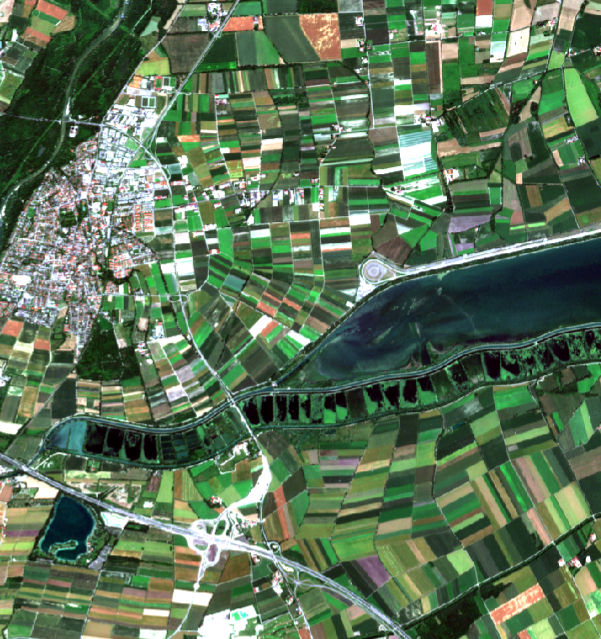
\includegraphics[width=\linewidth]{./Figures/munich_optical.png}
        \caption{Optical image}
        \label{fig:munich-o}
    \end{subfigure}
   \hspace{0.001\textwidth}
    \begin{subfigure}{0.315\textwidth}
        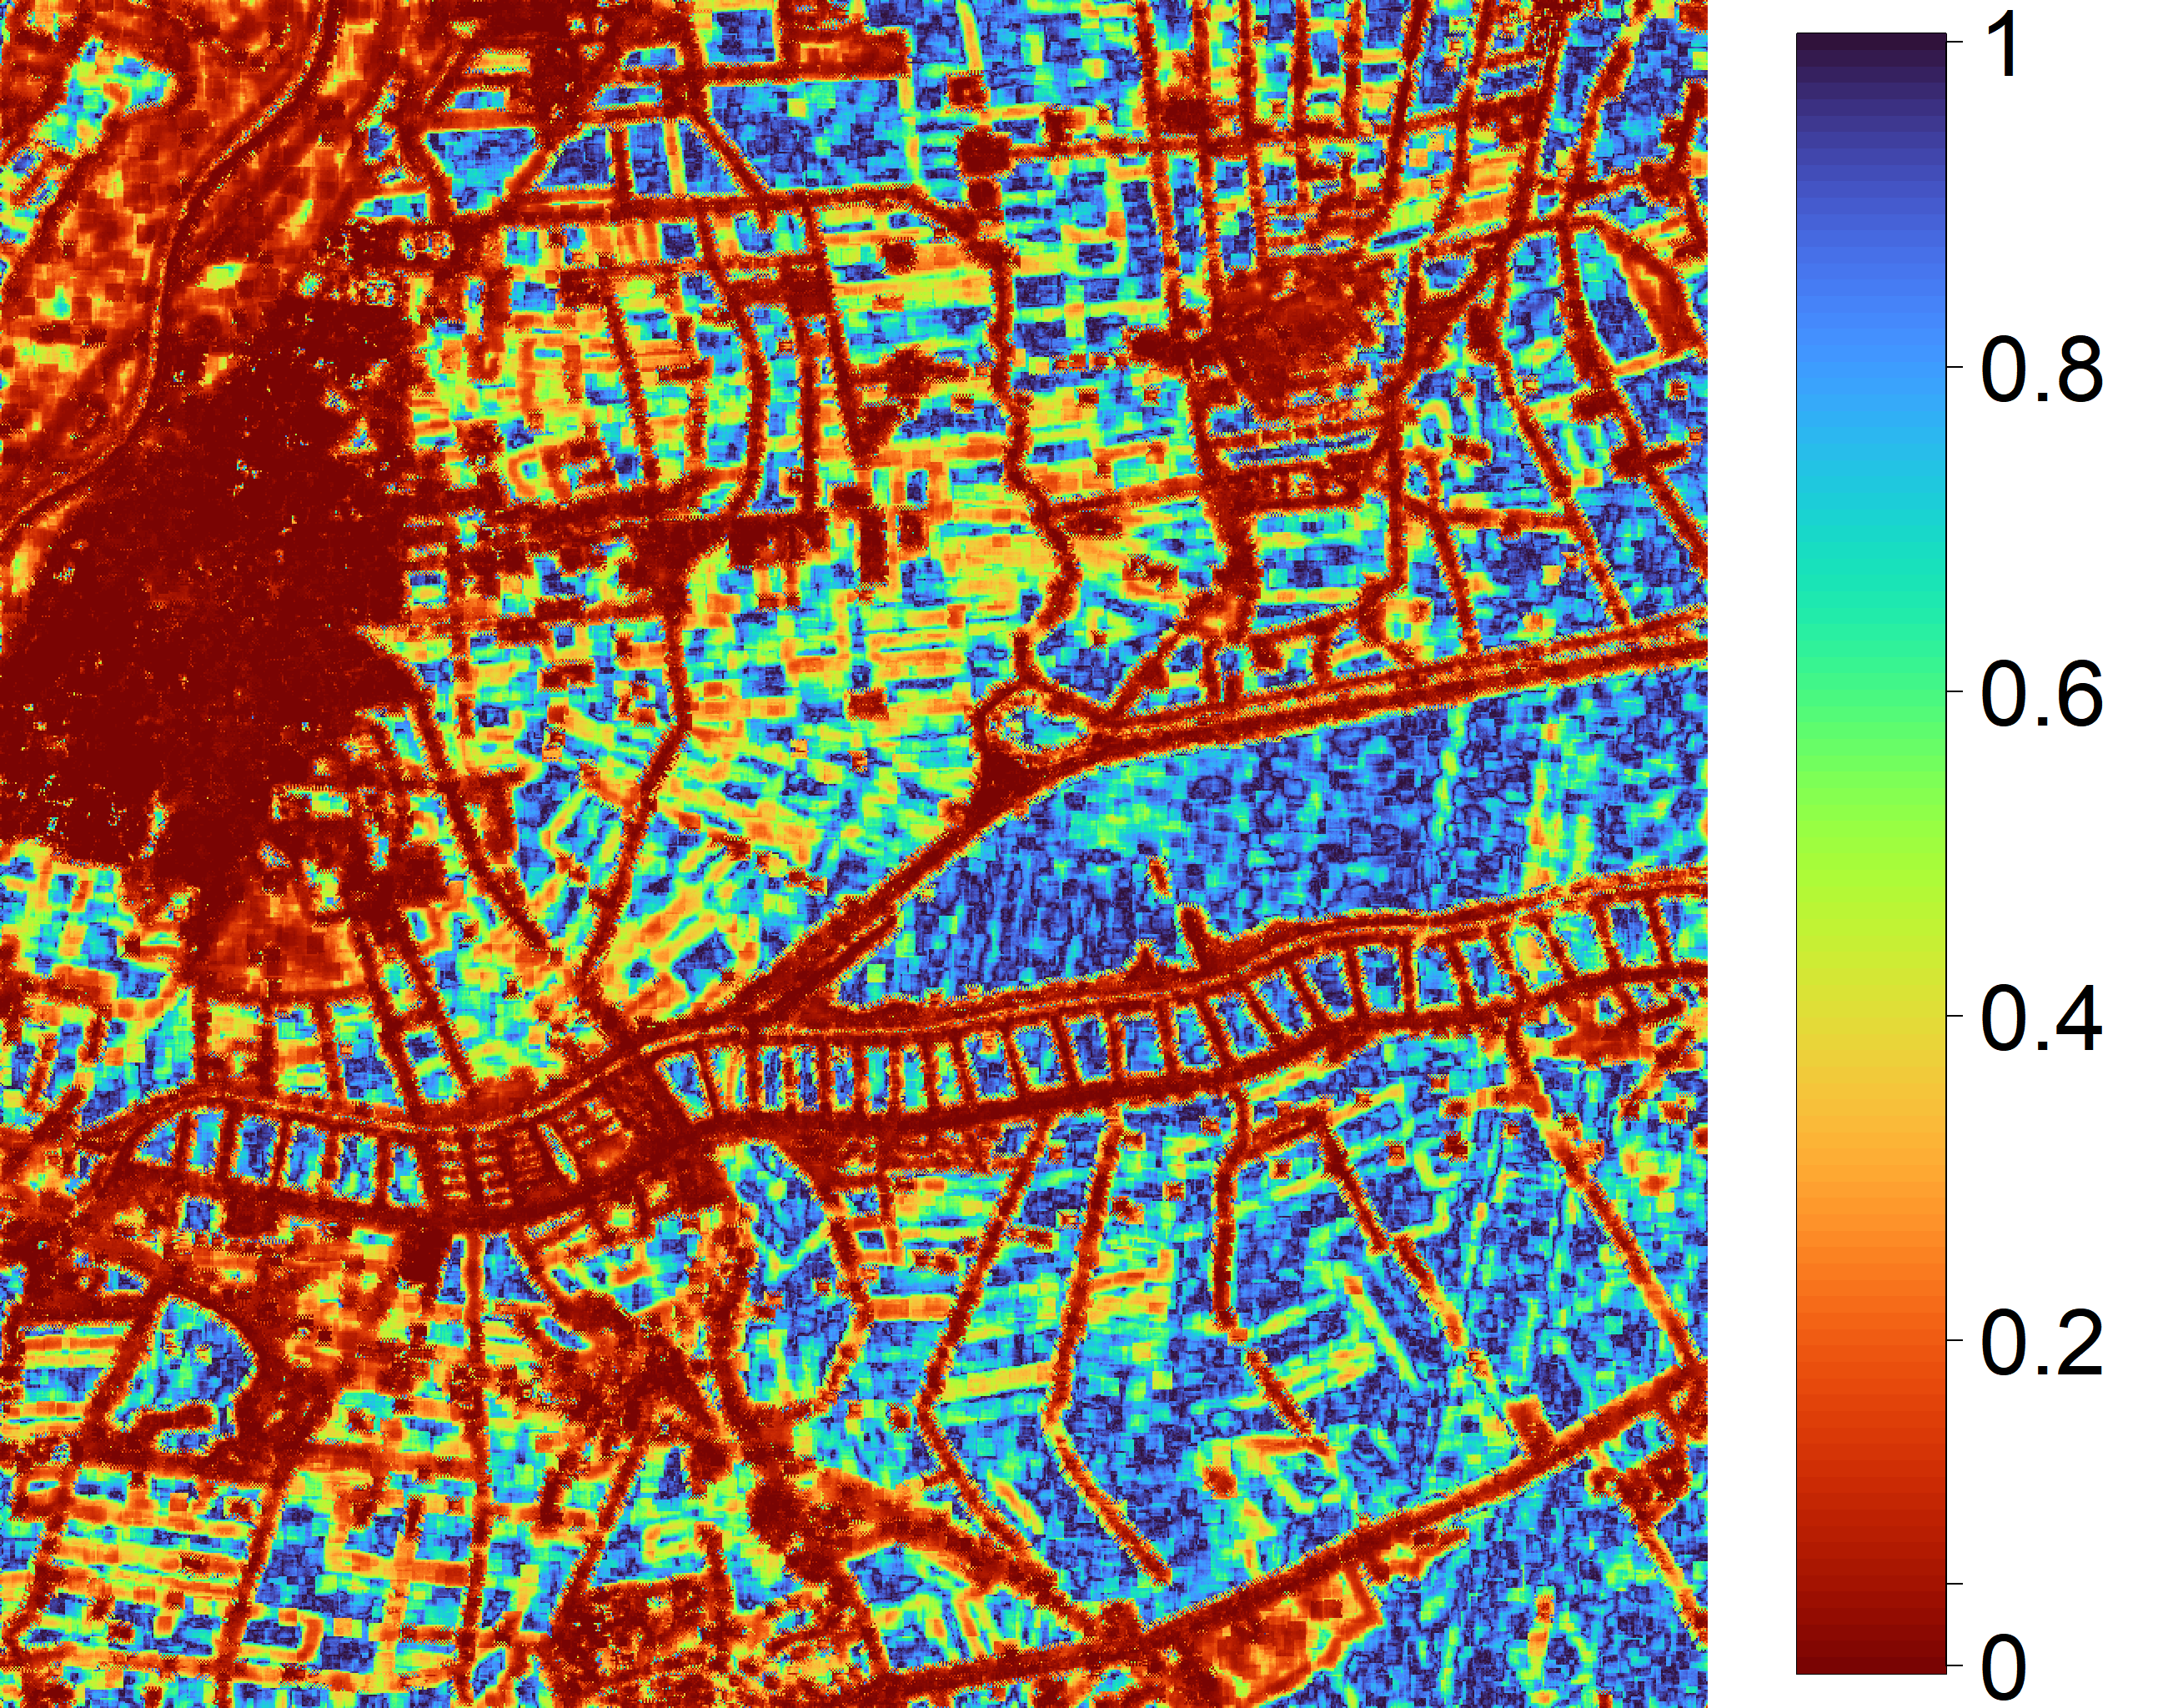
\includegraphics[width=\linewidth]{./Figures/p-values_munich50.png}
        \caption{$p$-value map   }
        \label{fig:munichp}
    \end{subfigure}
    \caption{Results on SAR data-Munich with the test $\small{S_{\widetilde{T}_{\lambda}}}$ and adaptive windows ($5\times5$ to $11\times11$). }
    \label{fig:munich}
\end{figure*}

\begin{figure*}[hbt]
    \centering
    \begin{subfigure}{0.25\textwidth}
        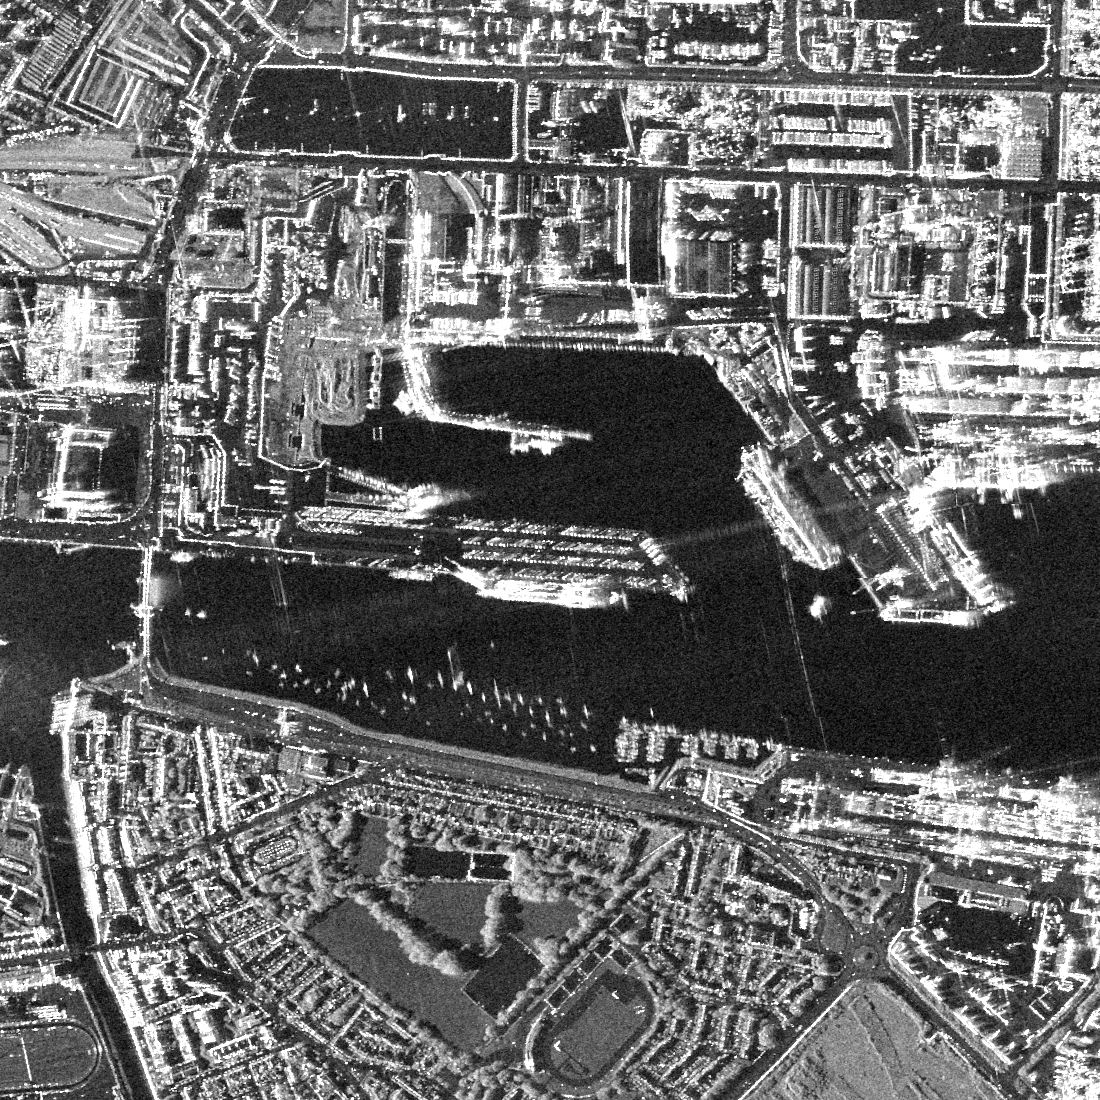
\includegraphics[width=\linewidth]{./Figures/dublin_1100_hh.png}
        \caption{Simulated image}
        \label{fig:dublin-sar}
    \end{subfigure}
    \hspace{0.00001\textwidth}
    \begin{subfigure}{0.25\textwidth}
        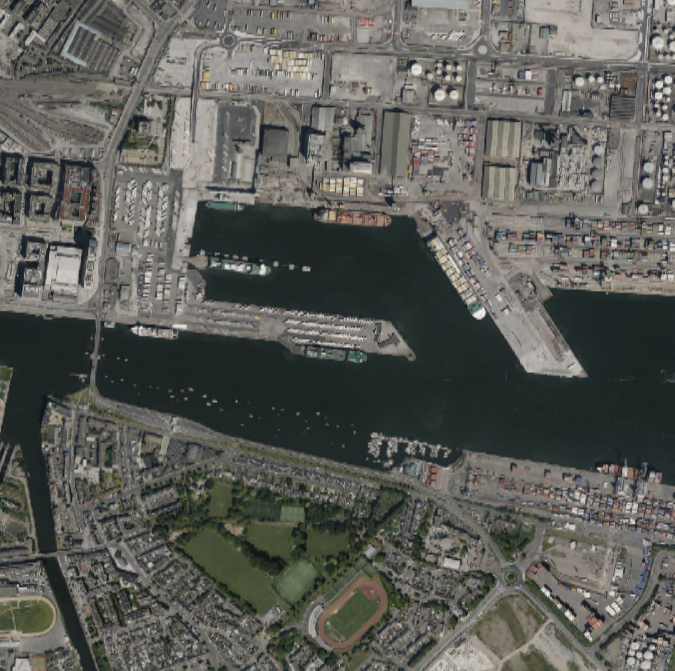
\includegraphics[width=\linewidth]{./Figures/dublin.png}
        \caption{Optical image   }
        \label{fig:dublin-o}
    \end{subfigure}
   \hspace{0.00001\textwidth}
    \begin{subfigure}{0.31\textwidth}
        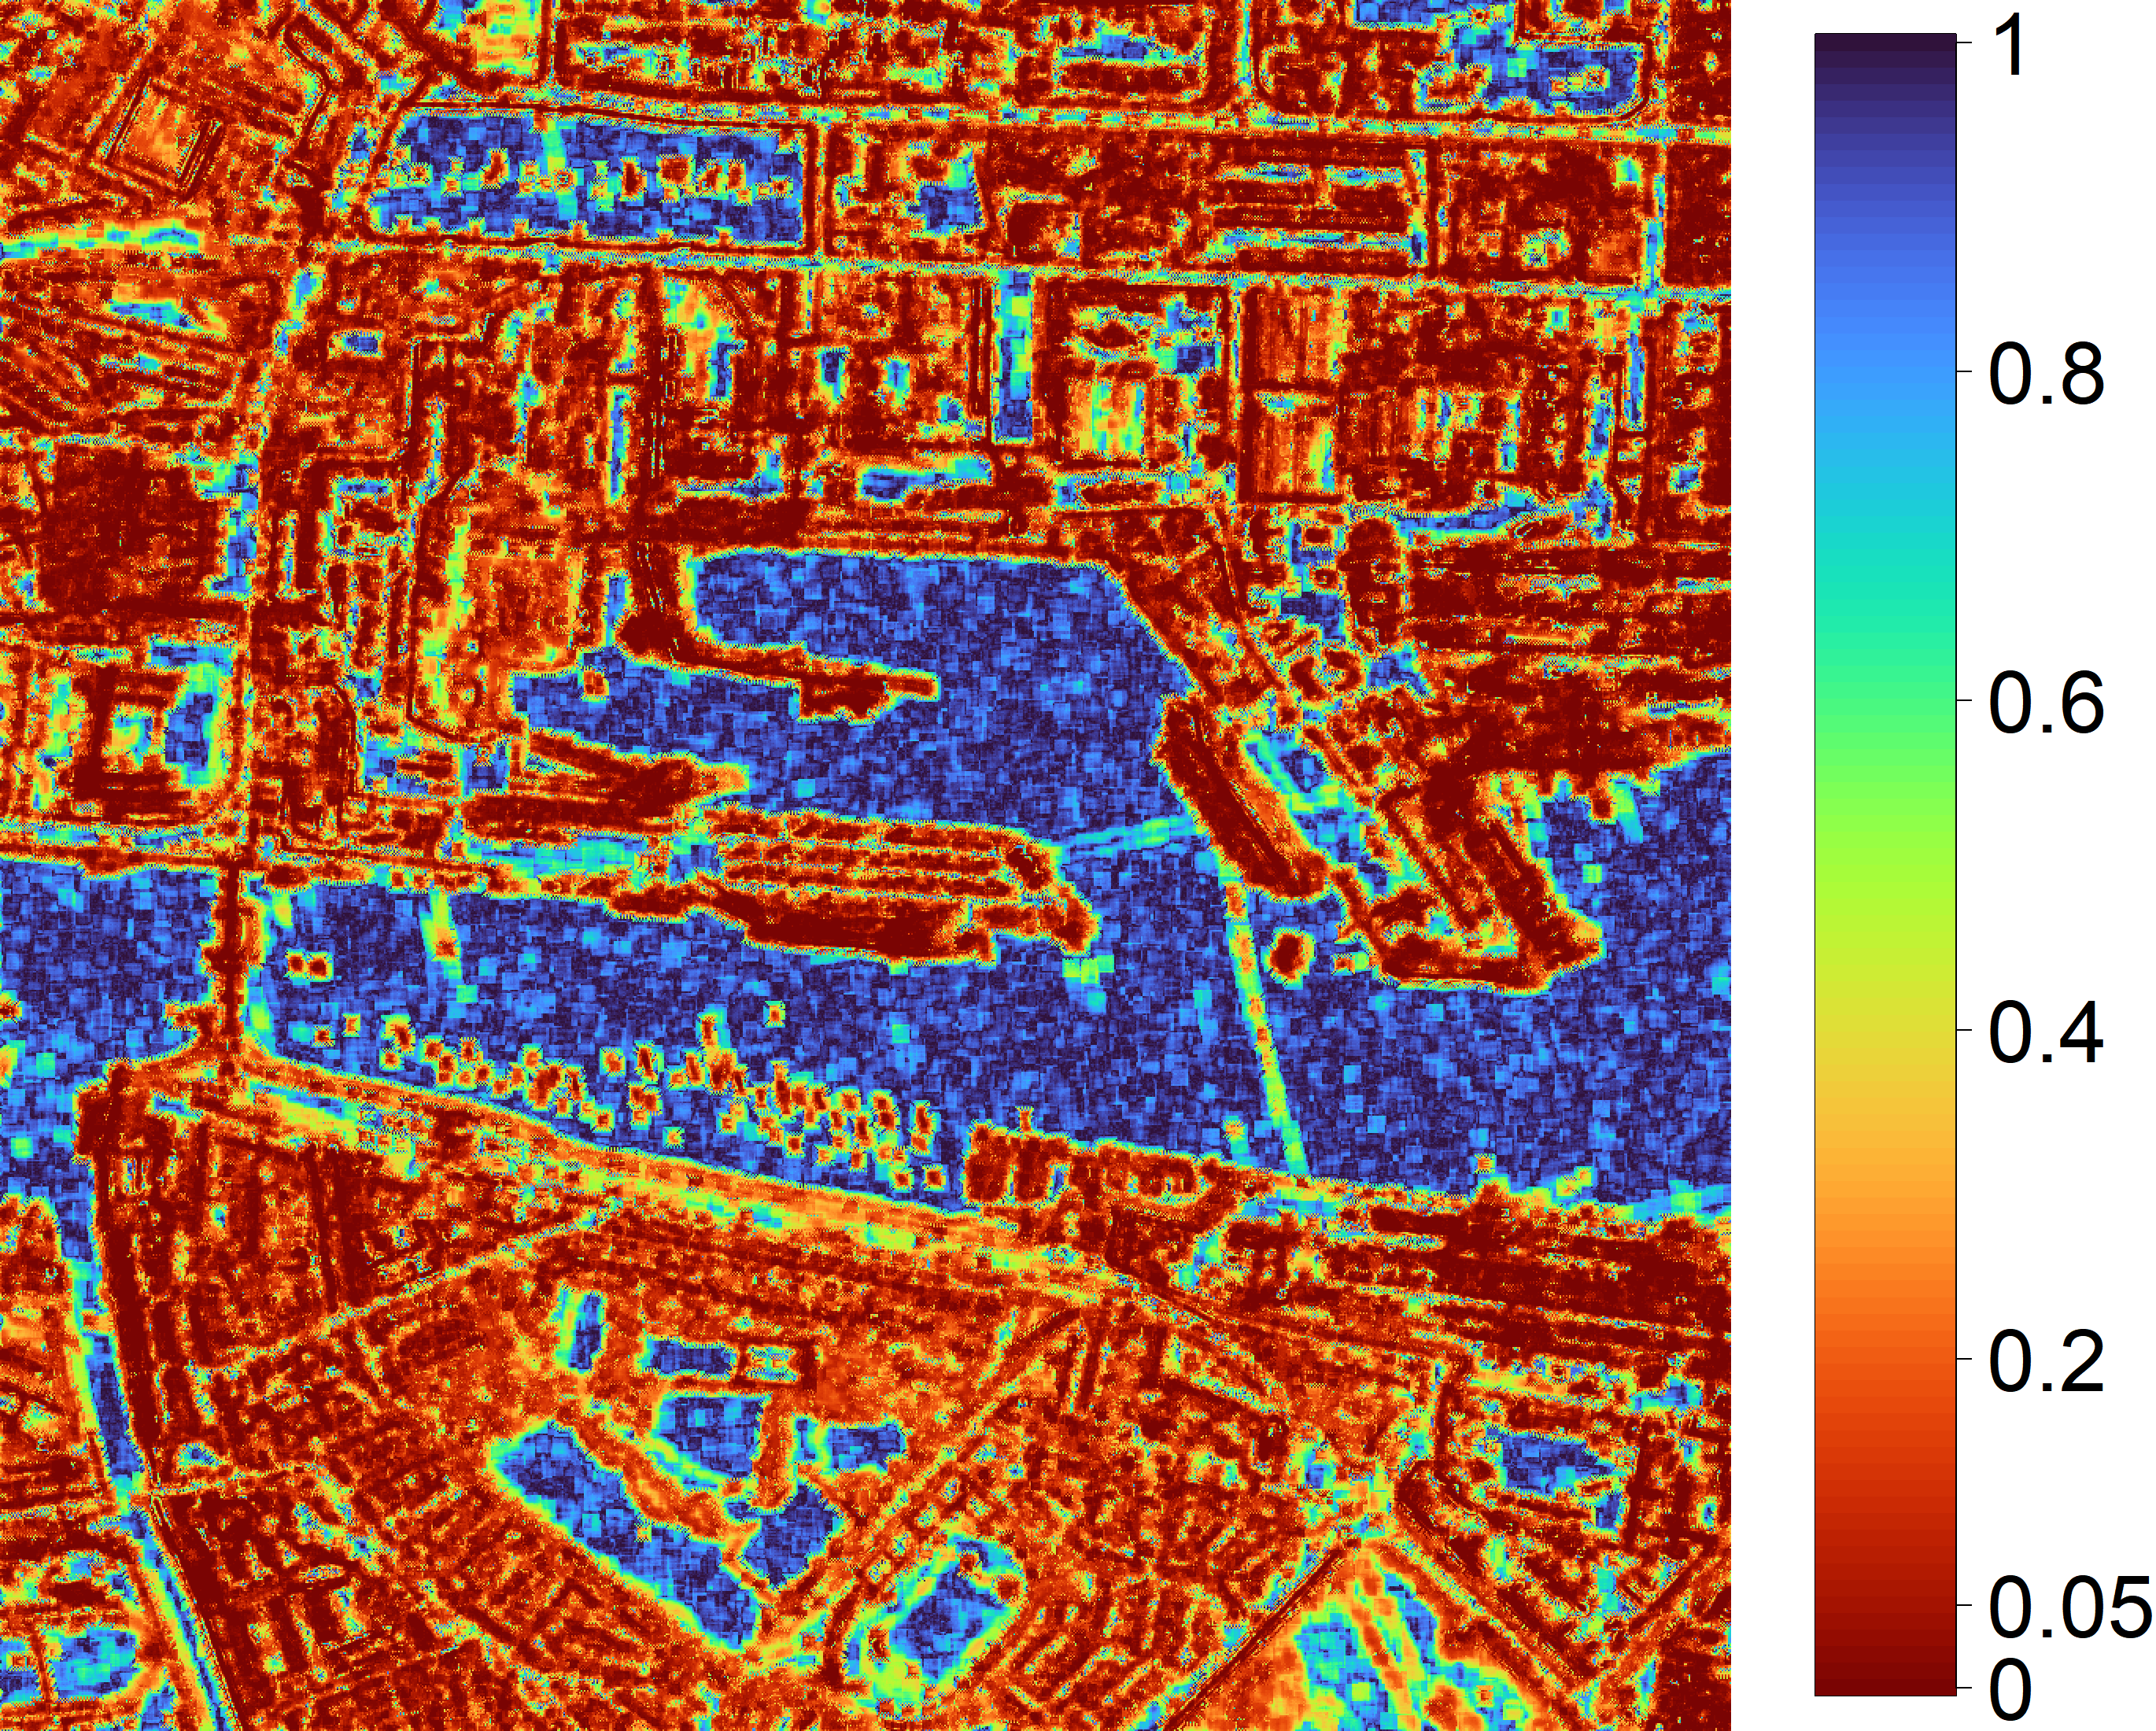
\includegraphics[width=\linewidth]{./Figures/p-values_dublin5v1.png}
        \caption{$p$-value map   }
        \label{fig:dublinp}
    \end{subfigure}
   \caption{Results on SAR data-Dublin with the test $\small{S_{\widetilde{T}_{\lambda}}}$ and adaptive windows ($5\times5$ to $11\times11$). }
    \label{fig:dublin}
\end{figure*}

The \(p\)-value maps provide a clear separation between homogeneous and
heterogeneous areas. Dark-red tones (\(p < 0.05\)) cluster around highly
textured features, including urban blocks, industrial and harbor
facilities, and road networks. These regions exhibit strong departures
from homogeneity, consistent with the expected scattering variability in
built environments. Intermediate tones (green and yellow,
\(0.2 < p < 0.6\)) appear in semi-structured areas such as agricultural
fields and mixed land covers, reflecting moderate texture. By contrast,
blue tones (\(p \approx 1\)) dominate in smooth regions such as open
water bodies, uniform pastures, and large homogeneous crop zones, where
the data behave in accordance with the null hypothesis.

The adaptive nature of the windowing plays a key role in these results.
Larger windows are automatically selected in homogeneous regions,
enhancing stability and noise suppression, while smaller windows are
used in heterogeneous areas, ensuring edge preservation and avoiding
class mixing. This balance allows the method to capture fine-scale
details such as canals, field boundaries, and narrow urban structures,
while still providing robust detection of broader homogeneous areas.

\section{Conclusions}\label{sec:conclusion}

\section*{References}\label{references}
\addcontentsline{toc}{section}{References}

\phantomsection\label{refs}
\begin{CSLReferences}{0}{0}
\bibitem[\citeproctext]{ref-Mondini2021}
\CSLLeftMargin{{[}1{]} }%
\CSLRightInline{A. C. Mondini, F. Guzzetti, K.-T. Chang, O. Monserrat,
T. R. Martha, and A. Manconi,
{``\href{https://doi.org/10.1016/j.earscirev.2021.103574}{Landslide
failures detection and mapping using synthetic aperture radar: Past,
present and future},''} \emph{Earth-Science Reviews}, vol. 216, p.
103574, 2021. }

\bibitem[\citeproctext]{ref-Zeng2020}
\CSLLeftMargin{{[}2{]} }%
\CSLRightInline{Z. Zeng \emph{et al.},
{``\href{https://doi.org/10.1016/j.jhydrol.2019.124377}{Towards high
resolution flood monitoring: An integrated methodology using passive
microwave brightness temperatures and sentinel synthetic aperture radar
imagery},''} \emph{Journal of Hydrology}, vol. 582, p. 124377, 2020. }

\bibitem[\citeproctext]{ref-Akbarizadeh2012}
\CSLLeftMargin{{[}3{]} }%
\CSLRightInline{G. Akbarizadeh,
{``\href{https://doi.org/10.1109/tgrs.2012.2194787}{A new
statistical-based kurtosis wavelet energy feature for texture
recognition of SAR images},''} \emph{IEEE Transactions on Geoscience and
Remote Sensing}, vol. 50, no. 11, pp. 4358--4368, 2012. }

\bibitem[\citeproctext]{ref-Moreira2013}
\CSLLeftMargin{{[}4{]} }%
\CSLRightInline{A. Moreira, P. Prats-Iraola, M. Younis, G. Krieger, I.
Hajnsek, and K. P. Papathanassiou,
{``\href{https://doi.org/10.1109/mgrs.2013.2248301}{A tutorial on
synthetic aperture radar},''} \emph{IEEE Geoscience and Remote Sensing
Magazine}, vol. 1, no. 1, pp. 6--43, 2013. }

\bibitem[\citeproctext]{ref-Mu2019}
\CSLLeftMargin{{[}5{]} }%
\CSLRightInline{Y. Mu, B. Huang, Z. Pan, H. Yang, G. Hou, and J. Duan,
{``An enhanced high-order variational model based on speckle noise
removal with {\(G^0\)} distribution,''} \emph{IEEE Access}, vol. 7, pp.
104365--104379, 2019. }

\bibitem[\citeproctext]{ref-Yu2023}
\CSLLeftMargin{{[}6{]} }%
\CSLRightInline{H. Yu, X. Yin, Z. Liu, S. Zhou, C. Li, and H. Jiang,
{``\href{https://doi.org/10.1109/jstars.2023.3257548}{A novel
unsupervised evaluation metric based on heterogeneity features for SAR
image segmentation},''} \emph{IEEE Journal of Selected Topics in Applied
Earth Observations and Remote Sensing}, vol. 16, pp. 2851--2867, 2023. }

\bibitem[\citeproctext]{ref-Argenti2013}
\CSLLeftMargin{{[}7{]} }%
\CSLRightInline{F. Argenti, A. Lapini, T. Bianchi, and L. Alparone,
{``\href{https://doi.org/10.1109/mgrs.2013.2277512}{A tutorial on
speckle reduction in synthetic aperture radar images},''} \emph{IEEE
Geoscience and Remote Sensing Magazine}, vol. 1, no. 3, pp. 6--35, 2013.
}

\bibitem[\citeproctext]{ref-Choi2019}
\CSLLeftMargin{{[}8{]} }%
\CSLRightInline{H. Choi and J. Jeong,
{``\href{https://doi.org/10.3390/rs11101184}{Speckle noise reduction
technique for SAR images using statistical characteristics of speckle
noise and discrete wavelet transform},''} \emph{Remote Sensing}, vol.
11, no. 10, p. 1184, 2019. }

\bibitem[\citeproctext]{ref-Baraha2023}
\CSLLeftMargin{{[}9{]} }%
\CSLRightInline{S. Baraha and A. K. Sahoo,
{``\href{https://doi.org/10.1016/j.sigpro.2023.109156}{Synthetic
aperture radar image and its despeckling using variational methods: A
review of recent trends},''} \emph{Signal Processing}, vol. 212, p.
109156, 2023. }

\bibitem[\citeproctext]{ref-Frery1997}
\CSLLeftMargin{{[}10{]} }%
\CSLRightInline{A. C. Frery, H.-J. Muller, C. C. F. Yanasse, and S. J.
S. SantAnna, {``A model for extremely heterogeneous clutter,''}
\emph{{IEEE} Transactions on Geoscience and Remote Sensing}, vol. 35,
no. 3, pp. 648--659, 1997. }

\bibitem[\citeproctext]{ref-Ferreira2020}
\CSLLeftMargin{{[}11{]} }%
\CSLRightInline{J. De A. Ferreira and A. D. C. Nascimento, {``Shannon
entropy for the {\(\mathcal {G}^0_{I}\)} model: A new segmentation
approach,''} \emph{{IEEE} Journal of Selected Topics in Applied Earth
Observations and Remote Sensing}, vol. 13, pp. 2547--2553, 2020. }

\bibitem[\citeproctext]{ref-Shannon1948}
\CSLLeftMargin{{[}12{]} }%
\CSLRightInline{C. E. Shannon, {``A mathematical theory of
communication,''} \emph{The Bell System Technical Journal}, vol. 27, no.
3, pp. 379--423, 1948. }

\bibitem[\citeproctext]{ref-Tsallis1988}
\CSLLeftMargin{{[}13{]} }%
\CSLRightInline{C. Tsallis,
{``\href{https://doi.org/10.1007/bf01016429}{Possible generalization of
boltzmann-gibbs statistics},''} \emph{Journal of Statistical Physics},
vol. 52, no. 1--2, pp. 479--487, 1988. }

\bibitem[\citeproctext]{ref-Nascimento2014}
\CSLLeftMargin{{[}14{]} }%
\CSLRightInline{A. D. C. Nascimento, M. M. Horta, A. C. Frery, and R. J.
Cintra, {``Comparing edge detection methods based on stochastic
entropies and distances for {PolSAR} imagery,''} \emph{{IEEE} Journal of
Selected Topics in Applied Earth Observations and Remote Sensing}, vol.
7, no. 2, pp. 648--663, 2014. }

\bibitem[\citeproctext]{ref-Nobre2016}
\CSLLeftMargin{{[}15{]} }%
\CSLRightInline{R. H. Nobre, F. A. A. Rodrigues, R. C. P. Marques, J. S.
Nobre, J. F. S. R. Neto, and F. N. S. Medeiros,
{``\href{https://doi.org/10.1109/lsp.2016.2606760}{SAR image
segmentation with {R}ényi's entropy},''} \emph{IEEE Signal Processing
Letters}, vol. 23, no. 11, pp. 1551--1555, 2016. }

\bibitem[\citeproctext]{ref-Chan2022}
\CSLLeftMargin{{[}16{]} }%
\CSLRightInline{D. Chan, J. Gambini, and A. C. Frery,
{``\href{https://doi.org/10.3390/rs14030509}{Entropy-based non-local
means filter for single-look SAR speckle reduction},''} \emph{Remote
Sensing}, vol. 14, no. 3, p. 509, 2022. }

\bibitem[\citeproctext]{ref-Park1999}
\CSLLeftMargin{{[}17{]} }%
\CSLRightInline{J.-M. Park, W. J. Song, and W. A. Pearlman,
{``\href{https://doi.org/10.1049/ip-vis:19990550}{Speckle filtering of
SAR images based on adaptive windowing},''} \emph{IEE Proceedings -
Vision, Image, and Signal Processing}, vol. 146, no. 4, p. 191, 1999. }

\bibitem[\citeproctext]{ref-Nascimento2010}
\CSLLeftMargin{{[}18{]} }%
\CSLRightInline{A. D. C. Nascimento, R. J. Cintra, and A. C. Frery,
{``Hypothesis testing in speckled data with stochastic distances,''}
\emph{{IEEE} Transactions on Geoscience and Remote Sensing}, vol. 48,
no. 1, pp. 373--385, Jan. 2010. }

\bibitem[\citeproctext]{ref-Havrda1967}
\CSLLeftMargin{{[}19{]} }%
\CSLRightInline{J. Havrda and F. Charvát, {``Quantification method of
classification processes. Concept of structural \(a\)-entropy,''}
\emph{Kybernetika}, vol. 3, no. 1, pp. (30)--35, 1967 {[}Online{]}.
Available: \url{http://eudml.org/doc/28681}}

\bibitem[\citeproctext]{ref-vasicek1976test}
\CSLLeftMargin{{[}20{]} }%
\CSLRightInline{O. Vasicek, {``A test for normality based on sample
entropy,''} \emph{Journal of the Royal Statistical Society Series B:
Statistical Methodology}, vol. 38, no. 1, pp. 54--59, 1976. }

\bibitem[\citeproctext]{ref-Ebrahimi1994}
\CSLLeftMargin{{[}21{]} }%
\CSLRightInline{N. Ebrahimi, K. Pflughoeft, and E. S. Soofi, {``Two
measures of sample entropy,''} \emph{Statistics \& Probability Letters},
vol. 20, no. 3, pp. 225--234, 1994. }

\bibitem[\citeproctext]{ref-AlLabadi2024}
\CSLLeftMargin{{[}22{]} }%
\CSLRightInline{L. Al-Labadi, Z. Chu, and Y. Xu,
{``\href{https://doi.org/10.1007/s00180-024-01507-z}{Advancements in
{R}ényi entropy and divergence estimation for model assessment},''}
\emph{Computational Statistics}, 2024. }

\bibitem[\citeproctext]{ref-Frery2024}
\CSLLeftMargin{{[}23{]} }%
\CSLRightInline{A. C. Frery, J. Alpala, and A. D. C. Nascimento,
{``\href{https://doi.org/10.3390/rs16111973}{Identifying heterogeneity
in {SAR} data with new test statistics},''} \emph{Remote Sensing}, vol.
16, no. 11, p. 1973, 2024. }

\bibitem[\citeproctext]{ref-Alpala2024}
\CSLLeftMargin{{[}24{]} }%
\CSLRightInline{J. Alpala, A. D. C. Nascimento, and A. C. Frery,
{``\href{https://doi.org/10.1109/migars61408.2024.10544448}{Identifying
departures from the fully developed speckle hypothesis in intensity
{SAR} data with non-parametric estimation of the entropy},''} in
\emph{2024 {I}nternational {C}onference on {M}achine {I}ntelligence for
{G}eo{A}nalytics and {R}emote {S}ensing ({MIGARS})}, 2024, pp. 1--4. }

\bibitem[\citeproctext]{ref-Alpala2025}
\CSLLeftMargin{{[}25{]} }%
\CSLRightInline{J. Alpala, A. D. C. Nascimento, and A. C. Frery,
{``\href{https://doi.org/10.1109/lgrs.2025.3581855}{Quantifying
heterogeneity in SAR imagery with the rényi entropy},''} \emph{IEEE
Geoscience and Remote Sensing Letters}, pp. 1--1, 2025. }

\bibitem[\citeproctext]{ref-VanEs1992}
\CSLLeftMargin{{[}26{]} }%
\CSLRightInline{B. Van Es, {``Estimating functionals related to a
density by a class of statistics based on spacings,''}
\emph{Scandinavian Journal of Statistics}, vol. 19, pp. 61--72, 1992. }

\bibitem[\citeproctext]{ref-Gomez2017}
\CSLLeftMargin{{[}27{]} }%
\CSLRightInline{L. Gomez, L. Alvarez, L. Mazorra, and A. C. Frery,
{``\href{https://doi.org/10.1016/j.neucom.2016.08.140}{Fully PolSAR
image classification using machine learning techniques and
reaction-diffusion systems},''} \emph{Neurocomputing}, vol. 255, pp.
52--60, 2017. }

\bibitem[\citeproctext]{ref-Frery2019a}
\CSLLeftMargin{{[}28{]} }%
\CSLRightInline{A. C. Frery and J. Gambini,
{``\href{https://doi.org/10.1007/s11749-019-00658-2}{Comparing samples
from the \({\mathcal {G}}^0\) distribution using a geodesic
distance},''} \emph{TEST}, vol. 29, no. 2, pp. 359--378, 2019. }

\bibitem[\citeproctext]{ref-Neto2023}
\CSLLeftMargin{{[}29{]} }%
\CSLRightInline{J. F. S. R. Neto and F. A. A. Rodrigues,
{``\href{https://doi.org/10.1109/lgrs.2023.3305119}{Improving
log-cumulant-based estimation of heterogeneity information in {SAR}
imagery},''} \emph{{IEEE} Geoscience and Remote Sensing Letters}, vol.
20, pp. 1--5, 2023. }

\end{CSLReferences}


% Can use something like this to put references on a page
% by themselves when using endfloat and the captionsoff option.
\ifCLASSOPTIONcaptionsoff
  \newpage
\fi

% trigger a \newpage just before the given reference
% number - used to balance the columns on the last page
% adjust value as needed - may need to be readjusted if
% the document is modified later
%\IEEEtriggeratref{8}
% The "triggered" command can be changed if desired:
%\IEEEtriggercmd{\enlargethispage{-5in}}

% Uncomment when use biblatex with style=ieee
%\renewcommand{\bibfont}{\footnotesize} % for IEEE bibfont size

\pagebreak[3]
% that's all folks
\end{document}

